%-*-latex-*-
\sectionthree{Heapify-down}
\begin{python0}
from solutions import *; clear()
\end{python0}

Heapify-down is the opposite of heapify-up:
you keep pushing a value \verb!v! down, swapping with the largest child
if that largest child is greater than \verb!v!. 
Here's an example.

Suppose I have this tree:

\begin{center}
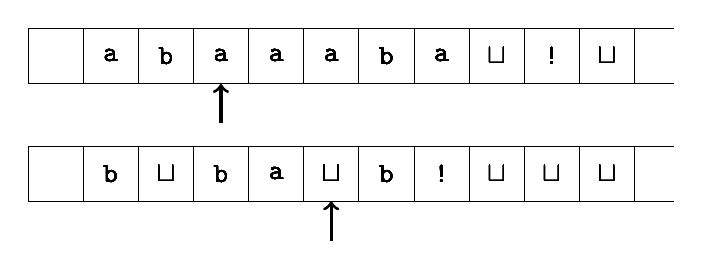
\begin{tikzpicture}

\draw (0.35, 0.35)
  node[draw, line width=0.01cm, , color=black,
       rounded corners=0cm, inner sep=0cm] {

\begin{minipage}[t][0.7cm]{0.7cm}
\mbox{}

\end{minipage}

};\draw (0.35, 0.35) node[color=black] {\texttt{\DOLLAR}};
\draw (1.0499999999999998, 0.35)
  node[draw, line width=0.01cm, , color=black,
       rounded corners=0cm, inner sep=0cm] {

\begin{minipage}[t][0.7cm]{0.7cm}
\mbox{}

\end{minipage}

};\draw (1.0499999999999998, 0.35) node[color=black] {\texttt{a}};
\draw (1.7499999999999998, 0.35)
  node[draw, line width=0.01cm, , color=black,
       rounded corners=0cm, inner sep=0cm] {

\begin{minipage}[t][0.7cm]{0.7cm}
\mbox{}

\end{minipage}

};\draw (1.7499999999999998, 0.35) node[color=black] {\texttt{b}};
\draw (2.4499999999999997, 0.35)
  node[draw, line width=0.01cm, , color=black,
       rounded corners=0cm, inner sep=0cm] {

\begin{minipage}[t][0.7cm]{0.7cm}
\mbox{}

\end{minipage}

};\draw (2.4499999999999997, 0.35) node[color=black] {\texttt{a}};
\draw (3.15, 0.35)
  node[draw, line width=0.01cm, , color=black,
       rounded corners=0cm, inner sep=0cm] {

\begin{minipage}[t][0.7cm]{0.7cm}
\mbox{}

\end{minipage}

};\draw (3.15, 0.35) node[color=black] {\texttt{a}};
\draw (3.85, 0.35)
  node[draw, line width=0.01cm, , color=black,
       rounded corners=0cm, inner sep=0cm] {

\begin{minipage}[t][0.7cm]{0.7cm}
\mbox{}

\end{minipage}

};\draw (3.85, 0.35) node[color=black] {\texttt{a}};
\draw (4.550000000000001, 0.35)
  node[draw, line width=0.01cm, , color=black,
       rounded corners=0cm, inner sep=0cm] {

\begin{minipage}[t][0.7cm]{0.7cm}
\mbox{}

\end{minipage}

};\draw (4.550000000000001, 0.35) node[color=black] {\texttt{b}};
\draw (5.25, 0.35)
  node[draw, line width=0.01cm, , color=black,
       rounded corners=0cm, inner sep=0cm] {

\begin{minipage}[t][0.7cm]{0.7cm}
\mbox{}

\end{minipage}

};\draw (5.25, 0.35) node[color=black] {\texttt{a}};
\draw (5.950000000000001, 0.35)
  node[draw, line width=0.01cm, , color=black,
       rounded corners=0cm, inner sep=0cm] {

\begin{minipage}[t][0.7cm]{0.7cm}
\mbox{}

\end{minipage}

};\draw (5.950000000000001, 0.35) node[color=black] {\texttt{$\sqcup$}};
\draw (6.65, 0.35)
  node[draw, line width=0.01cm, , color=black,
       rounded corners=0cm, inner sep=0cm] {

\begin{minipage}[t][0.7cm]{0.7cm}
\mbox{}

\end{minipage}

};\draw (6.65, 0.35) node[color=black] {\texttt{!}};
\draw (7.350000000000001, 0.35)
  node[draw, line width=0.01cm, , color=black,
       rounded corners=0cm, inner sep=0cm] {

\begin{minipage}[t][0.7cm]{0.7cm}
\mbox{}

\end{minipage}

};\draw (7.350000000000001, 0.35) node[color=black] {\texttt{$\sqcup$}};
\draw (0.35, 0.35)
  node[draw, line width=0.01cm, , color=black,
       rounded corners=0cm, inner sep=0cm] {

\begin{minipage}[t][0.7cm]{0.7cm}
\mbox{}

\end{minipage}

};\draw (0.35, 0.35) node[color=black] {\texttt{\DOLLAR}};
\draw (1.0499999999999998, 0.35)
  node[draw, line width=0.01cm, , color=black,
       rounded corners=0cm, inner sep=0cm] {

\begin{minipage}[t][0.7cm]{0.7cm}
\mbox{}

\end{minipage}

};\draw (1.0499999999999998, 0.35) node[color=black] {\texttt{a}};
\draw (1.7499999999999998, 0.35)
  node[draw, line width=0.01cm, , color=black,
       rounded corners=0cm, inner sep=0cm] {

\begin{minipage}[t][0.7cm]{0.7cm}
\mbox{}

\end{minipage}

};\draw (1.7499999999999998, 0.35) node[color=black] {\texttt{b}};
\draw (2.4499999999999997, 0.35)
  node[draw, line width=0.01cm, , color=black,
       rounded corners=0cm, inner sep=0cm] {

\begin{minipage}[t][0.7cm]{0.7cm}
\mbox{}

\end{minipage}

};\draw (2.4499999999999997, 0.35) node[color=black] {\texttt{a}};
\draw (3.15, 0.35)
  node[draw, line width=0.01cm, , color=black,
       rounded corners=0cm, inner sep=0cm] {

\begin{minipage}[t][0.7cm]{0.7cm}
\mbox{}

\end{minipage}

};\draw (3.15, 0.35) node[color=black] {\texttt{a}};
\draw (3.85, 0.35)
  node[draw, line width=0.01cm, , color=black,
       rounded corners=0cm, inner sep=0cm] {

\begin{minipage}[t][0.7cm]{0.7cm}
\mbox{}

\end{minipage}

};\draw (3.85, 0.35) node[color=black] {\texttt{a}};
\draw (4.550000000000001, 0.35)
  node[draw, line width=0.01cm, , color=black,
       rounded corners=0cm, inner sep=0cm] {

\begin{minipage}[t][0.7cm]{0.7cm}
\mbox{}

\end{minipage}

};\draw (4.550000000000001, 0.35) node[color=black] {\texttt{b}};
\draw (5.25, 0.35)
  node[draw, line width=0.01cm, , color=black,
       rounded corners=0cm, inner sep=0cm] {

\begin{minipage}[t][0.7cm]{0.7cm}
\mbox{}

\end{minipage}

};\draw (5.25, 0.35) node[color=black] {\texttt{a}};
\draw (5.950000000000001, 0.35)
  node[draw, line width=0.01cm, , color=black,
       rounded corners=0cm, inner sep=0cm] {

\begin{minipage}[t][0.7cm]{0.7cm}
\mbox{}

\end{minipage}

};\draw (5.950000000000001, 0.35) node[color=black] {\texttt{$\sqcup$}};
\draw (6.65, 0.35)
  node[draw, line width=0.01cm, , color=black,
       rounded corners=0cm, inner sep=0cm] {

\begin{minipage}[t][0.7cm]{0.7cm}
\mbox{}

\end{minipage}

};\draw (6.65, 0.35) node[color=black] {\texttt{!}};
\draw (7.350000000000001, 0.35)
  node[draw, line width=0.01cm, , color=black,
       rounded corners=0cm, inner sep=0cm] {

\begin{minipage}[t][0.7cm]{0.7cm}
\mbox{}

\end{minipage}

};\draw (7.350000000000001, 0.35) node[color=black] {\texttt{$\sqcup$}};
\draw (0.35, 0.35)
  node[draw, line width=0.01cm, , color=black,
       rounded corners=0cm, inner sep=0cm] {

\begin{minipage}[t][0.7cm]{0.7cm}
\mbox{}

\end{minipage}

};\draw (0.35, 0.35) node[color=black] {\texttt{\DOLLAR}};
\draw (1.0499999999999998, 0.35)
  node[draw, line width=0.01cm, , color=black,
       rounded corners=0cm, inner sep=0cm] {

\begin{minipage}[t][0.7cm]{0.7cm}
\mbox{}

\end{minipage}

};\draw (1.0499999999999998, 0.35) node[color=black] {\texttt{a}};
\draw (1.7499999999999998, 0.35)
  node[draw, line width=0.01cm, , color=black,
       rounded corners=0cm, inner sep=0cm] {

\begin{minipage}[t][0.7cm]{0.7cm}
\mbox{}

\end{minipage}

};\draw (1.7499999999999998, 0.35) node[color=black] {\texttt{b}};
\draw (2.4499999999999997, 0.35)
  node[draw, line width=0.01cm, , color=black,
       rounded corners=0cm, inner sep=0cm] {

\begin{minipage}[t][0.7cm]{0.7cm}
\mbox{}

\end{minipage}

};\draw (2.4499999999999997, 0.35) node[color=black] {\texttt{a}};
\draw (3.15, 0.35)
  node[draw, line width=0.01cm, , color=black,
       rounded corners=0cm, inner sep=0cm] {

\begin{minipage}[t][0.7cm]{0.7cm}
\mbox{}

\end{minipage}

};\draw (3.15, 0.35) node[color=black] {\texttt{a}};
\draw (3.85, 0.35)
  node[draw, line width=0.01cm, , color=black,
       rounded corners=0cm, inner sep=0cm] {

\begin{minipage}[t][0.7cm]{0.7cm}
\mbox{}

\end{minipage}

};\draw (3.85, 0.35) node[color=black] {\texttt{a}};
\draw (4.550000000000001, 0.35)
  node[draw, line width=0.01cm, , color=black,
       rounded corners=0cm, inner sep=0cm] {

\begin{minipage}[t][0.7cm]{0.7cm}
\mbox{}

\end{minipage}

};\draw (4.550000000000001, 0.35) node[color=black] {\texttt{b}};
\draw (5.25, 0.35)
  node[draw, line width=0.01cm, , color=black,
       rounded corners=0cm, inner sep=0cm] {

\begin{minipage}[t][0.7cm]{0.7cm}
\mbox{}

\end{minipage}

};\draw (5.25, 0.35) node[color=black] {\texttt{a}};
\draw (5.950000000000001, 0.35)
  node[draw, line width=0.01cm, , color=black,
       rounded corners=0cm, inner sep=0cm] {

\begin{minipage}[t][0.7cm]{0.7cm}
\mbox{}

\end{minipage}

};\draw (5.950000000000001, 0.35) node[color=black] {\texttt{$\sqcup$}};
\draw (6.65, 0.35)
  node[draw, line width=0.01cm, , color=black,
       rounded corners=0cm, inner sep=0cm] {

\begin{minipage}[t][0.7cm]{0.7cm}
\mbox{}

\end{minipage}

};\draw (6.65, 0.35) node[color=black] {\texttt{!}};
\draw (7.350000000000001, 0.35)
  node[draw, line width=0.01cm, , color=black,
       rounded corners=0cm, inner sep=0cm] {

\begin{minipage}[t][0.7cm]{0.7cm}
\mbox{}

\end{minipage}

};\draw (7.350000000000001, 0.35) node[color=black] {\texttt{$\sqcup$}};
\draw (0.35, 0.35)
  node[draw, line width=0.01cm, , color=black,
       rounded corners=0cm, inner sep=0cm] {

\begin{minipage}[t][0.7cm]{0.7cm}
\mbox{}

\end{minipage}

};\draw (0.35, 0.35) node[color=black] {\texttt{\DOLLAR}};
\draw (1.0499999999999998, 0.35)
  node[draw, line width=0.01cm, , color=black,
       rounded corners=0cm, inner sep=0cm] {

\begin{minipage}[t][0.7cm]{0.7cm}
\mbox{}

\end{minipage}

};\draw (1.0499999999999998, 0.35) node[color=black] {\texttt{a}};
\draw (1.7499999999999998, 0.35)
  node[draw, line width=0.01cm, , color=black,
       rounded corners=0cm, inner sep=0cm] {

\begin{minipage}[t][0.7cm]{0.7cm}
\mbox{}

\end{minipage}

};\draw (1.7499999999999998, 0.35) node[color=black] {\texttt{b}};
\draw (2.4499999999999997, 0.35)
  node[draw, line width=0.01cm, , color=black,
       rounded corners=0cm, inner sep=0cm] {

\begin{minipage}[t][0.7cm]{0.7cm}
\mbox{}

\end{minipage}

};\draw (2.4499999999999997, 0.35) node[color=black] {\texttt{a}};
\draw (3.15, 0.35)
  node[draw, line width=0.01cm, , color=black,
       rounded corners=0cm, inner sep=0cm] {

\begin{minipage}[t][0.7cm]{0.7cm}
\mbox{}

\end{minipage}

};\draw (3.15, 0.35) node[color=black] {\texttt{a}};
\draw (3.85, 0.35)
  node[draw, line width=0.01cm, , color=black,
       rounded corners=0cm, inner sep=0cm] {

\begin{minipage}[t][0.7cm]{0.7cm}
\mbox{}

\end{minipage}

};\draw (3.85, 0.35) node[color=black] {\texttt{a}};
\draw (4.550000000000001, 0.35)
  node[draw, line width=0.01cm, , color=black,
       rounded corners=0cm, inner sep=0cm] {

\begin{minipage}[t][0.7cm]{0.7cm}
\mbox{}

\end{minipage}

};\draw (4.550000000000001, 0.35) node[color=black] {\texttt{b}};
\draw (5.25, 0.35)
  node[draw, line width=0.01cm, , color=black,
       rounded corners=0cm, inner sep=0cm] {

\begin{minipage}[t][0.7cm]{0.7cm}
\mbox{}

\end{minipage}

};\draw (5.25, 0.35) node[color=black] {\texttt{a}};
\draw (5.950000000000001, 0.35)
  node[draw, line width=0.01cm, , color=black,
       rounded corners=0cm, inner sep=0cm] {

\begin{minipage}[t][0.7cm]{0.7cm}
\mbox{}

\end{minipage}

};\draw (5.950000000000001, 0.35) node[color=black] {\texttt{$\sqcup$}};
\draw (6.65, 0.35)
  node[draw, line width=0.01cm, , color=black,
       rounded corners=0cm, inner sep=0cm] {

\begin{minipage}[t][0.7cm]{0.7cm}
\mbox{}

\end{minipage}

};\draw (6.65, 0.35) node[color=black] {\texttt{!}};
\draw (7.350000000000001, 0.35)
  node[draw, line width=0.01cm, , color=black,
       rounded corners=0cm, inner sep=0cm] {

\begin{minipage}[t][0.7cm]{0.7cm}
\mbox{}

\end{minipage}

};\draw (7.350000000000001, 0.35) node[color=black] {\texttt{$\sqcup$}};
\draw (0.35, 0.35)
  node[draw, line width=0.01cm, , color=black,
       rounded corners=0cm, inner sep=0cm] {

\begin{minipage}[t][0.7cm]{0.7cm}
\mbox{}

\end{minipage}

};\draw (0.35, 0.35) node[color=black] {\texttt{\DOLLAR}};
\draw (1.0499999999999998, 0.35)
  node[draw, line width=0.01cm, , color=black,
       rounded corners=0cm, inner sep=0cm] {

\begin{minipage}[t][0.7cm]{0.7cm}
\mbox{}

\end{minipage}

};\draw (1.0499999999999998, 0.35) node[color=black] {\texttt{a}};
\draw (1.7499999999999998, 0.35)
  node[draw, line width=0.01cm, , color=black,
       rounded corners=0cm, inner sep=0cm] {

\begin{minipage}[t][0.7cm]{0.7cm}
\mbox{}

\end{minipage}

};\draw (1.7499999999999998, 0.35) node[color=black] {\texttt{b}};
\draw (2.4499999999999997, 0.35)
  node[draw, line width=0.01cm, , color=black,
       rounded corners=0cm, inner sep=0cm] {

\begin{minipage}[t][0.7cm]{0.7cm}
\mbox{}

\end{minipage}

};\draw (2.4499999999999997, 0.35) node[color=black] {\texttt{a}};
\draw (3.15, 0.35)
  node[draw, line width=0.01cm, , color=black,
       rounded corners=0cm, inner sep=0cm] {

\begin{minipage}[t][0.7cm]{0.7cm}
\mbox{}

\end{minipage}

};\draw (3.15, 0.35) node[color=black] {\texttt{a}};
\draw (3.85, 0.35)
  node[draw, line width=0.01cm, , color=black,
       rounded corners=0cm, inner sep=0cm] {

\begin{minipage}[t][0.7cm]{0.7cm}
\mbox{}

\end{minipage}

};\draw (3.85, 0.35) node[color=black] {\texttt{a}};
\draw (4.550000000000001, 0.35)
  node[draw, line width=0.01cm, , color=black,
       rounded corners=0cm, inner sep=0cm] {

\begin{minipage}[t][0.7cm]{0.7cm}
\mbox{}

\end{minipage}

};\draw (4.550000000000001, 0.35) node[color=black] {\texttt{b}};
\draw (5.25, 0.35)
  node[draw, line width=0.01cm, , color=black,
       rounded corners=0cm, inner sep=0cm] {

\begin{minipage}[t][0.7cm]{0.7cm}
\mbox{}

\end{minipage}

};\draw (5.25, 0.35) node[color=black] {\texttt{a}};
\draw (5.950000000000001, 0.35)
  node[draw, line width=0.01cm, , color=black,
       rounded corners=0cm, inner sep=0cm] {

\begin{minipage}[t][0.7cm]{0.7cm}
\mbox{}

\end{minipage}

};\draw (5.950000000000001, 0.35) node[color=black] {\texttt{$\sqcup$}};
\draw (6.65, 0.35)
  node[draw, line width=0.01cm, , color=black,
       rounded corners=0cm, inner sep=0cm] {

\begin{minipage}[t][0.7cm]{0.7cm}
\mbox{}

\end{minipage}

};\draw (6.65, 0.35) node[color=black] {\texttt{!}};
\draw (7.350000000000001, 0.35)
  node[draw, line width=0.01cm, , color=black,
       rounded corners=0cm, inner sep=0cm] {

\begin{minipage}[t][0.7cm]{0.7cm}
\mbox{}

\end{minipage}

};\draw (7.350000000000001, 0.35) node[color=black] {\texttt{$\sqcup$}};
\draw (0.35, 0.35)
  node[draw, line width=0.01cm, , color=black,
       rounded corners=0cm, inner sep=0cm] {

\begin{minipage}[t][0.7cm]{0.7cm}
\mbox{}

\end{minipage}

};\draw (0.35, 0.35) node[color=black] {\texttt{\DOLLAR}};
\draw (1.0499999999999998, 0.35)
  node[draw, line width=0.01cm, , color=black,
       rounded corners=0cm, inner sep=0cm] {

\begin{minipage}[t][0.7cm]{0.7cm}
\mbox{}

\end{minipage}

};\draw (1.0499999999999998, 0.35) node[color=black] {\texttt{a}};
\draw (1.7499999999999998, 0.35)
  node[draw, line width=0.01cm, , color=black,
       rounded corners=0cm, inner sep=0cm] {

\begin{minipage}[t][0.7cm]{0.7cm}
\mbox{}

\end{minipage}

};\draw (1.7499999999999998, 0.35) node[color=black] {\texttt{b}};
\draw (2.4499999999999997, 0.35)
  node[draw, line width=0.01cm, , color=black,
       rounded corners=0cm, inner sep=0cm] {

\begin{minipage}[t][0.7cm]{0.7cm}
\mbox{}

\end{minipage}

};\draw (2.4499999999999997, 0.35) node[color=black] {\texttt{a}};
\draw (3.15, 0.35)
  node[draw, line width=0.01cm, , color=black,
       rounded corners=0cm, inner sep=0cm] {

\begin{minipage}[t][0.7cm]{0.7cm}
\mbox{}

\end{minipage}

};\draw (3.15, 0.35) node[color=black] {\texttt{a}};
\draw (3.85, 0.35)
  node[draw, line width=0.01cm, , color=black,
       rounded corners=0cm, inner sep=0cm] {

\begin{minipage}[t][0.7cm]{0.7cm}
\mbox{}

\end{minipage}

};\draw (3.85, 0.35) node[color=black] {\texttt{a}};
\draw (4.550000000000001, 0.35)
  node[draw, line width=0.01cm, , color=black,
       rounded corners=0cm, inner sep=0cm] {

\begin{minipage}[t][0.7cm]{0.7cm}
\mbox{}

\end{minipage}

};\draw (4.550000000000001, 0.35) node[color=black] {\texttt{b}};
\draw (5.25, 0.35)
  node[draw, line width=0.01cm, , color=black,
       rounded corners=0cm, inner sep=0cm] {

\begin{minipage}[t][0.7cm]{0.7cm}
\mbox{}

\end{minipage}

};\draw (5.25, 0.35) node[color=black] {\texttt{a}};
\draw (5.950000000000001, 0.35)
  node[draw, line width=0.01cm, , color=black,
       rounded corners=0cm, inner sep=0cm] {

\begin{minipage}[t][0.7cm]{0.7cm}
\mbox{}

\end{minipage}

};\draw (5.950000000000001, 0.35) node[color=black] {\texttt{$\sqcup$}};
\draw (6.65, 0.35)
  node[draw, line width=0.01cm, , color=black,
       rounded corners=0cm, inner sep=0cm] {

\begin{minipage}[t][0.7cm]{0.7cm}
\mbox{}

\end{minipage}

};\draw (6.65, 0.35) node[color=black] {\texttt{!}};
\draw (7.350000000000001, 0.35)
  node[draw, line width=0.01cm, , color=black,
       rounded corners=0cm, inner sep=0cm] {

\begin{minipage}[t][0.7cm]{0.7cm}
\mbox{}

\end{minipage}

};\draw (7.350000000000001, 0.35) node[color=black] {\texttt{$\sqcup$}};
\draw (0.35, 0.35)
  node[draw, line width=0.01cm, , color=black,
       rounded corners=0cm, inner sep=0cm] {

\begin{minipage}[t][0.7cm]{0.7cm}
\mbox{}

\end{minipage}

};\draw (0.35, 0.35) node[color=black] {\texttt{\DOLLAR}};
\draw (1.0499999999999998, 0.35)
  node[draw, line width=0.01cm, , color=black,
       rounded corners=0cm, inner sep=0cm] {

\begin{minipage}[t][0.7cm]{0.7cm}
\mbox{}

\end{minipage}

};\draw (1.0499999999999998, 0.35) node[color=black] {\texttt{a}};
\draw (1.7499999999999998, 0.35)
  node[draw, line width=0.01cm, , color=black,
       rounded corners=0cm, inner sep=0cm] {

\begin{minipage}[t][0.7cm]{0.7cm}
\mbox{}

\end{minipage}

};\draw (1.7499999999999998, 0.35) node[color=black] {\texttt{b}};
\draw (2.4499999999999997, 0.35)
  node[draw, line width=0.01cm, , color=black,
       rounded corners=0cm, inner sep=0cm] {

\begin{minipage}[t][0.7cm]{0.7cm}
\mbox{}

\end{minipage}

};\draw (2.4499999999999997, 0.35) node[color=black] {\texttt{a}};
\draw (3.15, 0.35)
  node[draw, line width=0.01cm, , color=black,
       rounded corners=0cm, inner sep=0cm] {

\begin{minipage}[t][0.7cm]{0.7cm}
\mbox{}

\end{minipage}

};\draw (3.15, 0.35) node[color=black] {\texttt{a}};
\draw (3.85, 0.35)
  node[draw, line width=0.01cm, , color=black,
       rounded corners=0cm, inner sep=0cm] {

\begin{minipage}[t][0.7cm]{0.7cm}
\mbox{}

\end{minipage}

};\draw (3.85, 0.35) node[color=black] {\texttt{a}};
\draw (4.550000000000001, 0.35)
  node[draw, line width=0.01cm, , color=black,
       rounded corners=0cm, inner sep=0cm] {

\begin{minipage}[t][0.7cm]{0.7cm}
\mbox{}

\end{minipage}

};\draw (4.550000000000001, 0.35) node[color=black] {\texttt{b}};
\draw (5.25, 0.35)
  node[draw, line width=0.01cm, , color=black,
       rounded corners=0cm, inner sep=0cm] {

\begin{minipage}[t][0.7cm]{0.7cm}
\mbox{}

\end{minipage}

};\draw (5.25, 0.35) node[color=black] {\texttt{a}};
\draw (5.950000000000001, 0.35)
  node[draw, line width=0.01cm, , color=black,
       rounded corners=0cm, inner sep=0cm] {

\begin{minipage}[t][0.7cm]{0.7cm}
\mbox{}

\end{minipage}

};\draw (5.950000000000001, 0.35) node[color=black] {\texttt{$\sqcup$}};
\draw (6.65, 0.35)
  node[draw, line width=0.01cm, , color=black,
       rounded corners=0cm, inner sep=0cm] {

\begin{minipage}[t][0.7cm]{0.7cm}
\mbox{}

\end{minipage}

};\draw (6.65, 0.35) node[color=black] {\texttt{!}};
\draw (7.350000000000001, 0.35)
  node[draw, line width=0.01cm, , color=black,
       rounded corners=0cm, inner sep=0cm] {

\begin{minipage}[t][0.7cm]{0.7cm}
\mbox{}

\end{minipage}

};\draw (7.350000000000001, 0.35) node[color=black] {\texttt{$\sqcup$}};
\draw (0.35, 0.35)
  node[draw, line width=0.01cm, , color=black,
       rounded corners=0cm, inner sep=0cm] {

\begin{minipage}[t][0.7cm]{0.7cm}
\mbox{}

\end{minipage}

};\draw (0.35, 0.35) node[color=black] {\texttt{\DOLLAR}};
\draw (1.0499999999999998, 0.35)
  node[draw, line width=0.01cm, , color=black,
       rounded corners=0cm, inner sep=0cm] {

\begin{minipage}[t][0.7cm]{0.7cm}
\mbox{}

\end{minipage}

};\draw (1.0499999999999998, 0.35) node[color=black] {\texttt{a}};
\draw (1.7499999999999998, 0.35)
  node[draw, line width=0.01cm, , color=black,
       rounded corners=0cm, inner sep=0cm] {

\begin{minipage}[t][0.7cm]{0.7cm}
\mbox{}

\end{minipage}

};\draw (1.7499999999999998, 0.35) node[color=black] {\texttt{b}};
\draw (2.4499999999999997, 0.35)
  node[draw, line width=0.01cm, , color=black,
       rounded corners=0cm, inner sep=0cm] {

\begin{minipage}[t][0.7cm]{0.7cm}
\mbox{}

\end{minipage}

};\draw (2.4499999999999997, 0.35) node[color=black] {\texttt{a}};
\draw (3.15, 0.35)
  node[draw, line width=0.01cm, , color=black,
       rounded corners=0cm, inner sep=0cm] {

\begin{minipage}[t][0.7cm]{0.7cm}
\mbox{}

\end{minipage}

};\draw (3.15, 0.35) node[color=black] {\texttt{a}};
\draw (3.85, 0.35)
  node[draw, line width=0.01cm, , color=black,
       rounded corners=0cm, inner sep=0cm] {

\begin{minipage}[t][0.7cm]{0.7cm}
\mbox{}

\end{minipage}

};\draw (3.85, 0.35) node[color=black] {\texttt{a}};
\draw (4.550000000000001, 0.35)
  node[draw, line width=0.01cm, , color=black,
       rounded corners=0cm, inner sep=0cm] {

\begin{minipage}[t][0.7cm]{0.7cm}
\mbox{}

\end{minipage}

};\draw (4.550000000000001, 0.35) node[color=black] {\texttt{b}};
\draw (5.25, 0.35)
  node[draw, line width=0.01cm, , color=black,
       rounded corners=0cm, inner sep=0cm] {

\begin{minipage}[t][0.7cm]{0.7cm}
\mbox{}

\end{minipage}

};\draw (5.25, 0.35) node[color=black] {\texttt{a}};
\draw (5.950000000000001, 0.35)
  node[draw, line width=0.01cm, , color=black,
       rounded corners=0cm, inner sep=0cm] {

\begin{minipage}[t][0.7cm]{0.7cm}
\mbox{}

\end{minipage}

};\draw (5.950000000000001, 0.35) node[color=black] {\texttt{$\sqcup$}};
\draw (6.65, 0.35)
  node[draw, line width=0.01cm, , color=black,
       rounded corners=0cm, inner sep=0cm] {

\begin{minipage}[t][0.7cm]{0.7cm}
\mbox{}

\end{minipage}

};\draw (6.65, 0.35) node[color=black] {\texttt{!}};
\draw (7.350000000000001, 0.35)
  node[draw, line width=0.01cm, , color=black,
       rounded corners=0cm, inner sep=0cm] {

\begin{minipage}[t][0.7cm]{0.7cm}
\mbox{}

\end{minipage}

};\draw (7.350000000000001, 0.35) node[color=black] {\texttt{$\sqcup$}};
\draw (0.35, 0.35)
  node[draw, line width=0.01cm, , color=black,
       rounded corners=0cm, inner sep=0cm] {

\begin{minipage}[t][0.7cm]{0.7cm}
\mbox{}

\end{minipage}

};\draw (0.35, 0.35) node[color=black] {\texttt{\DOLLAR}};
\draw (1.0499999999999998, 0.35)
  node[draw, line width=0.01cm, , color=black,
       rounded corners=0cm, inner sep=0cm] {

\begin{minipage}[t][0.7cm]{0.7cm}
\mbox{}

\end{minipage}

};\draw (1.0499999999999998, 0.35) node[color=black] {\texttt{a}};
\draw (1.7499999999999998, 0.35)
  node[draw, line width=0.01cm, , color=black,
       rounded corners=0cm, inner sep=0cm] {

\begin{minipage}[t][0.7cm]{0.7cm}
\mbox{}

\end{minipage}

};\draw (1.7499999999999998, 0.35) node[color=black] {\texttt{b}};
\draw (2.4499999999999997, 0.35)
  node[draw, line width=0.01cm, , color=black,
       rounded corners=0cm, inner sep=0cm] {

\begin{minipage}[t][0.7cm]{0.7cm}
\mbox{}

\end{minipage}

};\draw (2.4499999999999997, 0.35) node[color=black] {\texttt{a}};
\draw (3.15, 0.35)
  node[draw, line width=0.01cm, , color=black,
       rounded corners=0cm, inner sep=0cm] {

\begin{minipage}[t][0.7cm]{0.7cm}
\mbox{}

\end{minipage}

};\draw (3.15, 0.35) node[color=black] {\texttt{a}};
\draw (3.85, 0.35)
  node[draw, line width=0.01cm, , color=black,
       rounded corners=0cm, inner sep=0cm] {

\begin{minipage}[t][0.7cm]{0.7cm}
\mbox{}

\end{minipage}

};\draw (3.85, 0.35) node[color=black] {\texttt{a}};
\draw (4.550000000000001, 0.35)
  node[draw, line width=0.01cm, , color=black,
       rounded corners=0cm, inner sep=0cm] {

\begin{minipage}[t][0.7cm]{0.7cm}
\mbox{}

\end{minipage}

};\draw (4.550000000000001, 0.35) node[color=black] {\texttt{b}};
\draw (5.25, 0.35)
  node[draw, line width=0.01cm, , color=black,
       rounded corners=0cm, inner sep=0cm] {

\begin{minipage}[t][0.7cm]{0.7cm}
\mbox{}

\end{minipage}

};\draw (5.25, 0.35) node[color=black] {\texttt{a}};
\draw (5.950000000000001, 0.35)
  node[draw, line width=0.01cm, , color=black,
       rounded corners=0cm, inner sep=0cm] {

\begin{minipage}[t][0.7cm]{0.7cm}
\mbox{}

\end{minipage}

};\draw (5.950000000000001, 0.35) node[color=black] {\texttt{$\sqcup$}};
\draw (6.65, 0.35)
  node[draw, line width=0.01cm, , color=black,
       rounded corners=0cm, inner sep=0cm] {

\begin{minipage}[t][0.7cm]{0.7cm}
\mbox{}

\end{minipage}

};\draw (6.65, 0.35) node[color=black] {\texttt{!}};
\draw (7.350000000000001, 0.35)
  node[draw, line width=0.01cm, , color=black,
       rounded corners=0cm, inner sep=0cm] {

\begin{minipage}[t][0.7cm]{0.7cm}
\mbox{}

\end{minipage}

};\draw (7.350000000000001, 0.35) node[color=black] {\texttt{$\sqcup$}};
\draw (0.35, 0.35)
  node[draw, line width=0.01cm, , color=black,
       rounded corners=0cm, inner sep=0cm] {

\begin{minipage}[t][0.7cm]{0.7cm}
\mbox{}

\end{minipage}

};\draw (0.35, 0.35) node[color=black] {\texttt{\DOLLAR}};
\draw (1.0499999999999998, 0.35)
  node[draw, line width=0.01cm, , color=black,
       rounded corners=0cm, inner sep=0cm] {

\begin{minipage}[t][0.7cm]{0.7cm}
\mbox{}

\end{minipage}

};\draw (1.0499999999999998, 0.35) node[color=black] {\texttt{a}};
\draw (1.7499999999999998, 0.35)
  node[draw, line width=0.01cm, , color=black,
       rounded corners=0cm, inner sep=0cm] {

\begin{minipage}[t][0.7cm]{0.7cm}
\mbox{}

\end{minipage}

};\draw (1.7499999999999998, 0.35) node[color=black] {\texttt{b}};
\draw (2.4499999999999997, 0.35)
  node[draw, line width=0.01cm, , color=black,
       rounded corners=0cm, inner sep=0cm] {

\begin{minipage}[t][0.7cm]{0.7cm}
\mbox{}

\end{minipage}

};\draw (2.4499999999999997, 0.35) node[color=black] {\texttt{a}};
\draw (3.15, 0.35)
  node[draw, line width=0.01cm, , color=black,
       rounded corners=0cm, inner sep=0cm] {

\begin{minipage}[t][0.7cm]{0.7cm}
\mbox{}

\end{minipage}

};\draw (3.15, 0.35) node[color=black] {\texttt{a}};
\draw (3.85, 0.35)
  node[draw, line width=0.01cm, , color=black,
       rounded corners=0cm, inner sep=0cm] {

\begin{minipage}[t][0.7cm]{0.7cm}
\mbox{}

\end{minipage}

};\draw (3.85, 0.35) node[color=black] {\texttt{a}};
\draw (4.550000000000001, 0.35)
  node[draw, line width=0.01cm, , color=black,
       rounded corners=0cm, inner sep=0cm] {

\begin{minipage}[t][0.7cm]{0.7cm}
\mbox{}

\end{minipage}

};\draw (4.550000000000001, 0.35) node[color=black] {\texttt{b}};
\draw (5.25, 0.35)
  node[draw, line width=0.01cm, , color=black,
       rounded corners=0cm, inner sep=0cm] {

\begin{minipage}[t][0.7cm]{0.7cm}
\mbox{}

\end{minipage}

};\draw (5.25, 0.35) node[color=black] {\texttt{a}};
\draw (5.950000000000001, 0.35)
  node[draw, line width=0.01cm, , color=black,
       rounded corners=0cm, inner sep=0cm] {

\begin{minipage}[t][0.7cm]{0.7cm}
\mbox{}

\end{minipage}

};\draw (5.950000000000001, 0.35) node[color=black] {\texttt{$\sqcup$}};
\draw (6.65, 0.35)
  node[draw, line width=0.01cm, , color=black,
       rounded corners=0cm, inner sep=0cm] {

\begin{minipage}[t][0.7cm]{0.7cm}
\mbox{}

\end{minipage}

};\draw (6.65, 0.35) node[color=black] {\texttt{!}};
\draw (7.350000000000001, 0.35)
  node[draw, line width=0.01cm, , color=black,
       rounded corners=0cm, inner sep=0cm] {

\begin{minipage}[t][0.7cm]{0.7cm}
\mbox{}

\end{minipage}

};\draw (7.350000000000001, 0.35) node[color=black] {\texttt{$\sqcup$}};
\draw (0.35, 0.35)
  node[draw, line width=0.01cm, , color=black,
       rounded corners=0cm, inner sep=0cm] {

\begin{minipage}[t][0.7cm]{0.7cm}
\mbox{}

\end{minipage}

};\draw (0.35, 0.35) node[color=black] {\texttt{\DOLLAR}};
\draw (1.0499999999999998, 0.35)
  node[draw, line width=0.01cm, , color=black,
       rounded corners=0cm, inner sep=0cm] {

\begin{minipage}[t][0.7cm]{0.7cm}
\mbox{}

\end{minipage}

};\draw (1.0499999999999998, 0.35) node[color=black] {\texttt{a}};
\draw (1.7499999999999998, 0.35)
  node[draw, line width=0.01cm, , color=black,
       rounded corners=0cm, inner sep=0cm] {

\begin{minipage}[t][0.7cm]{0.7cm}
\mbox{}

\end{minipage}

};\draw (1.7499999999999998, 0.35) node[color=black] {\texttt{b}};
\draw (2.4499999999999997, 0.35)
  node[draw, line width=0.01cm, , color=black,
       rounded corners=0cm, inner sep=0cm] {

\begin{minipage}[t][0.7cm]{0.7cm}
\mbox{}

\end{minipage}

};\draw (2.4499999999999997, 0.35) node[color=black] {\texttt{a}};
\draw (3.15, 0.35)
  node[draw, line width=0.01cm, , color=black,
       rounded corners=0cm, inner sep=0cm] {

\begin{minipage}[t][0.7cm]{0.7cm}
\mbox{}

\end{minipage}

};\draw (3.15, 0.35) node[color=black] {\texttt{a}};
\draw (3.85, 0.35)
  node[draw, line width=0.01cm, , color=black,
       rounded corners=0cm, inner sep=0cm] {

\begin{minipage}[t][0.7cm]{0.7cm}
\mbox{}

\end{minipage}

};\draw (3.85, 0.35) node[color=black] {\texttt{a}};
\draw (4.550000000000001, 0.35)
  node[draw, line width=0.01cm, , color=black,
       rounded corners=0cm, inner sep=0cm] {

\begin{minipage}[t][0.7cm]{0.7cm}
\mbox{}

\end{minipage}

};\draw (4.550000000000001, 0.35) node[color=black] {\texttt{b}};
\draw (5.25, 0.35)
  node[draw, line width=0.01cm, , color=black,
       rounded corners=0cm, inner sep=0cm] {

\begin{minipage}[t][0.7cm]{0.7cm}
\mbox{}

\end{minipage}

};\draw (5.25, 0.35) node[color=black] {\texttt{a}};
\draw (5.950000000000001, 0.35)
  node[draw, line width=0.01cm, , color=black,
       rounded corners=0cm, inner sep=0cm] {

\begin{minipage}[t][0.7cm]{0.7cm}
\mbox{}

\end{minipage}

};\draw (5.950000000000001, 0.35) node[color=black] {\texttt{$\sqcup$}};
\draw (6.65, 0.35)
  node[draw, line width=0.01cm, , color=black,
       rounded corners=0cm, inner sep=0cm] {

\begin{minipage}[t][0.7cm]{0.7cm}
\mbox{}

\end{minipage}

};\draw (6.65, 0.35) node[color=black] {\texttt{!}};
\draw (7.350000000000001, 0.35)
  node[draw, line width=0.01cm, , color=black,
       rounded corners=0cm, inner sep=0cm] {

\begin{minipage}[t][0.7cm]{0.7cm}
\mbox{}

\end{minipage}

};\draw (7.350000000000001, 0.35) node[color=black] {\texttt{$\sqcup$}};\draw[line width=0.01cm,black] (7.700000000000001,0.7) to  (8.200000000000001,0.7);
\draw[line width=0.01cm,black] (7.700000000000001,0.0) to  (8.200000000000001,0.0);
\draw[line width=0.04cm,black,->] (2.45,-0.51) to  (2.45,-0.01);

\draw (0.35, -1.15)
  node[draw, line width=0.01cm, , color=black,
       rounded corners=0cm, inner sep=0cm] {

\begin{minipage}[t][0.7cm]{0.7cm}
\mbox{}

\end{minipage}

};\draw (0.35, -1.15) node[color=black] {\texttt{\DOLLAR}};
\draw (1.0499999999999998, -1.15)
  node[draw, line width=0.01cm, , color=black,
       rounded corners=0cm, inner sep=0cm] {

\begin{minipage}[t][0.7cm]{0.7cm}
\mbox{}

\end{minipage}

};\draw (1.0499999999999998, -1.15) node[color=black] {\texttt{b}};
\draw (1.7499999999999998, -1.15)
  node[draw, line width=0.01cm, , color=black,
       rounded corners=0cm, inner sep=0cm] {

\begin{minipage}[t][0.7cm]{0.7cm}
\mbox{}

\end{minipage}

};\draw (1.7499999999999998, -1.15) node[color=black] {\texttt{$\sqcup$}};
\draw (2.4499999999999997, -1.15)
  node[draw, line width=0.01cm, , color=black,
       rounded corners=0cm, inner sep=0cm] {

\begin{minipage}[t][0.7cm]{0.7cm}
\mbox{}

\end{minipage}

};\draw (2.4499999999999997, -1.15) node[color=black] {\texttt{b}};
\draw (3.15, -1.15)
  node[draw, line width=0.01cm, , color=black,
       rounded corners=0cm, inner sep=0cm] {

\begin{minipage}[t][0.7cm]{0.7cm}
\mbox{}

\end{minipage}

};\draw (3.15, -1.15) node[color=black] {\texttt{a}};
\draw (3.85, -1.15)
  node[draw, line width=0.01cm, , color=black,
       rounded corners=0cm, inner sep=0cm] {

\begin{minipage}[t][0.7cm]{0.7cm}
\mbox{}

\end{minipage}

};\draw (3.85, -1.15) node[color=black] {\texttt{$\sqcup$}};
\draw (4.550000000000001, -1.15)
  node[draw, line width=0.01cm, , color=black,
       rounded corners=0cm, inner sep=0cm] {

\begin{minipage}[t][0.7cm]{0.7cm}
\mbox{}

\end{minipage}

};\draw (4.550000000000001, -1.15) node[color=black] {\texttt{b}};
\draw (5.25, -1.15)
  node[draw, line width=0.01cm, , color=black,
       rounded corners=0cm, inner sep=0cm] {

\begin{minipage}[t][0.7cm]{0.7cm}
\mbox{}

\end{minipage}

};\draw (5.25, -1.15) node[color=black] {\texttt{!}};
\draw (5.950000000000001, -1.15)
  node[draw, line width=0.01cm, , color=black,
       rounded corners=0cm, inner sep=0cm] {

\begin{minipage}[t][0.7cm]{0.7cm}
\mbox{}

\end{minipage}

};\draw (5.950000000000001, -1.15) node[color=black] {\texttt{$\sqcup$}};
\draw (6.65, -1.15)
  node[draw, line width=0.01cm, , color=black,
       rounded corners=0cm, inner sep=0cm] {

\begin{minipage}[t][0.7cm]{0.7cm}
\mbox{}

\end{minipage}

};\draw (6.65, -1.15) node[color=black] {\texttt{$\sqcup$}};
\draw (7.350000000000001, -1.15)
  node[draw, line width=0.01cm, , color=black,
       rounded corners=0cm, inner sep=0cm] {

\begin{minipage}[t][0.7cm]{0.7cm}
\mbox{}

\end{minipage}

};\draw (7.350000000000001, -1.15) node[color=black] {\texttt{$\sqcup$}};
\draw (0.35, -1.15)
  node[draw, line width=0.01cm, , color=black,
       rounded corners=0cm, inner sep=0cm] {

\begin{minipage}[t][0.7cm]{0.7cm}
\mbox{}

\end{minipage}

};\draw (0.35, -1.15) node[color=black] {\texttt{\DOLLAR}};
\draw (1.0499999999999998, -1.15)
  node[draw, line width=0.01cm, , color=black,
       rounded corners=0cm, inner sep=0cm] {

\begin{minipage}[t][0.7cm]{0.7cm}
\mbox{}

\end{minipage}

};\draw (1.0499999999999998, -1.15) node[color=black] {\texttt{b}};
\draw (1.7499999999999998, -1.15)
  node[draw, line width=0.01cm, , color=black,
       rounded corners=0cm, inner sep=0cm] {

\begin{minipage}[t][0.7cm]{0.7cm}
\mbox{}

\end{minipage}

};\draw (1.7499999999999998, -1.15) node[color=black] {\texttt{$\sqcup$}};
\draw (2.4499999999999997, -1.15)
  node[draw, line width=0.01cm, , color=black,
       rounded corners=0cm, inner sep=0cm] {

\begin{minipage}[t][0.7cm]{0.7cm}
\mbox{}

\end{minipage}

};\draw (2.4499999999999997, -1.15) node[color=black] {\texttt{b}};
\draw (3.15, -1.15)
  node[draw, line width=0.01cm, , color=black,
       rounded corners=0cm, inner sep=0cm] {

\begin{minipage}[t][0.7cm]{0.7cm}
\mbox{}

\end{minipage}

};\draw (3.15, -1.15) node[color=black] {\texttt{a}};
\draw (3.85, -1.15)
  node[draw, line width=0.01cm, , color=black,
       rounded corners=0cm, inner sep=0cm] {

\begin{minipage}[t][0.7cm]{0.7cm}
\mbox{}

\end{minipage}

};\draw (3.85, -1.15) node[color=black] {\texttt{$\sqcup$}};
\draw (4.550000000000001, -1.15)
  node[draw, line width=0.01cm, , color=black,
       rounded corners=0cm, inner sep=0cm] {

\begin{minipage}[t][0.7cm]{0.7cm}
\mbox{}

\end{minipage}

};\draw (4.550000000000001, -1.15) node[color=black] {\texttt{b}};
\draw (5.25, -1.15)
  node[draw, line width=0.01cm, , color=black,
       rounded corners=0cm, inner sep=0cm] {

\begin{minipage}[t][0.7cm]{0.7cm}
\mbox{}

\end{minipage}

};\draw (5.25, -1.15) node[color=black] {\texttt{!}};
\draw (5.950000000000001, -1.15)
  node[draw, line width=0.01cm, , color=black,
       rounded corners=0cm, inner sep=0cm] {

\begin{minipage}[t][0.7cm]{0.7cm}
\mbox{}

\end{minipage}

};\draw (5.950000000000001, -1.15) node[color=black] {\texttt{$\sqcup$}};
\draw (6.65, -1.15)
  node[draw, line width=0.01cm, , color=black,
       rounded corners=0cm, inner sep=0cm] {

\begin{minipage}[t][0.7cm]{0.7cm}
\mbox{}

\end{minipage}

};\draw (6.65, -1.15) node[color=black] {\texttt{$\sqcup$}};
\draw (7.350000000000001, -1.15)
  node[draw, line width=0.01cm, , color=black,
       rounded corners=0cm, inner sep=0cm] {

\begin{minipage}[t][0.7cm]{0.7cm}
\mbox{}

\end{minipage}

};\draw (7.350000000000001, -1.15) node[color=black] {\texttt{$\sqcup$}};
\draw (0.35, -1.15)
  node[draw, line width=0.01cm, , color=black,
       rounded corners=0cm, inner sep=0cm] {

\begin{minipage}[t][0.7cm]{0.7cm}
\mbox{}

\end{minipage}

};\draw (0.35, -1.15) node[color=black] {\texttt{\DOLLAR}};
\draw (1.0499999999999998, -1.15)
  node[draw, line width=0.01cm, , color=black,
       rounded corners=0cm, inner sep=0cm] {

\begin{minipage}[t][0.7cm]{0.7cm}
\mbox{}

\end{minipage}

};\draw (1.0499999999999998, -1.15) node[color=black] {\texttt{b}};
\draw (1.7499999999999998, -1.15)
  node[draw, line width=0.01cm, , color=black,
       rounded corners=0cm, inner sep=0cm] {

\begin{minipage}[t][0.7cm]{0.7cm}
\mbox{}

\end{minipage}

};\draw (1.7499999999999998, -1.15) node[color=black] {\texttt{$\sqcup$}};
\draw (2.4499999999999997, -1.15)
  node[draw, line width=0.01cm, , color=black,
       rounded corners=0cm, inner sep=0cm] {

\begin{minipage}[t][0.7cm]{0.7cm}
\mbox{}

\end{minipage}

};\draw (2.4499999999999997, -1.15) node[color=black] {\texttt{b}};
\draw (3.15, -1.15)
  node[draw, line width=0.01cm, , color=black,
       rounded corners=0cm, inner sep=0cm] {

\begin{minipage}[t][0.7cm]{0.7cm}
\mbox{}

\end{minipage}

};\draw (3.15, -1.15) node[color=black] {\texttt{a}};
\draw (3.85, -1.15)
  node[draw, line width=0.01cm, , color=black,
       rounded corners=0cm, inner sep=0cm] {

\begin{minipage}[t][0.7cm]{0.7cm}
\mbox{}

\end{minipage}

};\draw (3.85, -1.15) node[color=black] {\texttt{$\sqcup$}};
\draw (4.550000000000001, -1.15)
  node[draw, line width=0.01cm, , color=black,
       rounded corners=0cm, inner sep=0cm] {

\begin{minipage}[t][0.7cm]{0.7cm}
\mbox{}

\end{minipage}

};\draw (4.550000000000001, -1.15) node[color=black] {\texttt{b}};
\draw (5.25, -1.15)
  node[draw, line width=0.01cm, , color=black,
       rounded corners=0cm, inner sep=0cm] {

\begin{minipage}[t][0.7cm]{0.7cm}
\mbox{}

\end{minipage}

};\draw (5.25, -1.15) node[color=black] {\texttt{!}};
\draw (5.950000000000001, -1.15)
  node[draw, line width=0.01cm, , color=black,
       rounded corners=0cm, inner sep=0cm] {

\begin{minipage}[t][0.7cm]{0.7cm}
\mbox{}

\end{minipage}

};\draw (5.950000000000001, -1.15) node[color=black] {\texttt{$\sqcup$}};
\draw (6.65, -1.15)
  node[draw, line width=0.01cm, , color=black,
       rounded corners=0cm, inner sep=0cm] {

\begin{minipage}[t][0.7cm]{0.7cm}
\mbox{}

\end{minipage}

};\draw (6.65, -1.15) node[color=black] {\texttt{$\sqcup$}};
\draw (7.350000000000001, -1.15)
  node[draw, line width=0.01cm, , color=black,
       rounded corners=0cm, inner sep=0cm] {

\begin{minipage}[t][0.7cm]{0.7cm}
\mbox{}

\end{minipage}

};\draw (7.350000000000001, -1.15) node[color=black] {\texttt{$\sqcup$}};
\draw (0.35, -1.15)
  node[draw, line width=0.01cm, , color=black,
       rounded corners=0cm, inner sep=0cm] {

\begin{minipage}[t][0.7cm]{0.7cm}
\mbox{}

\end{minipage}

};\draw (0.35, -1.15) node[color=black] {\texttt{\DOLLAR}};
\draw (1.0499999999999998, -1.15)
  node[draw, line width=0.01cm, , color=black,
       rounded corners=0cm, inner sep=0cm] {

\begin{minipage}[t][0.7cm]{0.7cm}
\mbox{}

\end{minipage}

};\draw (1.0499999999999998, -1.15) node[color=black] {\texttt{b}};
\draw (1.7499999999999998, -1.15)
  node[draw, line width=0.01cm, , color=black,
       rounded corners=0cm, inner sep=0cm] {

\begin{minipage}[t][0.7cm]{0.7cm}
\mbox{}

\end{minipage}

};\draw (1.7499999999999998, -1.15) node[color=black] {\texttt{$\sqcup$}};
\draw (2.4499999999999997, -1.15)
  node[draw, line width=0.01cm, , color=black,
       rounded corners=0cm, inner sep=0cm] {

\begin{minipage}[t][0.7cm]{0.7cm}
\mbox{}

\end{minipage}

};\draw (2.4499999999999997, -1.15) node[color=black] {\texttt{b}};
\draw (3.15, -1.15)
  node[draw, line width=0.01cm, , color=black,
       rounded corners=0cm, inner sep=0cm] {

\begin{minipage}[t][0.7cm]{0.7cm}
\mbox{}

\end{minipage}

};\draw (3.15, -1.15) node[color=black] {\texttt{a}};
\draw (3.85, -1.15)
  node[draw, line width=0.01cm, , color=black,
       rounded corners=0cm, inner sep=0cm] {

\begin{minipage}[t][0.7cm]{0.7cm}
\mbox{}

\end{minipage}

};\draw (3.85, -1.15) node[color=black] {\texttt{$\sqcup$}};
\draw (4.550000000000001, -1.15)
  node[draw, line width=0.01cm, , color=black,
       rounded corners=0cm, inner sep=0cm] {

\begin{minipage}[t][0.7cm]{0.7cm}
\mbox{}

\end{minipage}

};\draw (4.550000000000001, -1.15) node[color=black] {\texttt{b}};
\draw (5.25, -1.15)
  node[draw, line width=0.01cm, , color=black,
       rounded corners=0cm, inner sep=0cm] {

\begin{minipage}[t][0.7cm]{0.7cm}
\mbox{}

\end{minipage}

};\draw (5.25, -1.15) node[color=black] {\texttt{!}};
\draw (5.950000000000001, -1.15)
  node[draw, line width=0.01cm, , color=black,
       rounded corners=0cm, inner sep=0cm] {

\begin{minipage}[t][0.7cm]{0.7cm}
\mbox{}

\end{minipage}

};\draw (5.950000000000001, -1.15) node[color=black] {\texttt{$\sqcup$}};
\draw (6.65, -1.15)
  node[draw, line width=0.01cm, , color=black,
       rounded corners=0cm, inner sep=0cm] {

\begin{minipage}[t][0.7cm]{0.7cm}
\mbox{}

\end{minipage}

};\draw (6.65, -1.15) node[color=black] {\texttt{$\sqcup$}};
\draw (7.350000000000001, -1.15)
  node[draw, line width=0.01cm, , color=black,
       rounded corners=0cm, inner sep=0cm] {

\begin{minipage}[t][0.7cm]{0.7cm}
\mbox{}

\end{minipage}

};\draw (7.350000000000001, -1.15) node[color=black] {\texttt{$\sqcup$}};
\draw (0.35, -1.15)
  node[draw, line width=0.01cm, , color=black,
       rounded corners=0cm, inner sep=0cm] {

\begin{minipage}[t][0.7cm]{0.7cm}
\mbox{}

\end{minipage}

};\draw (0.35, -1.15) node[color=black] {\texttt{\DOLLAR}};
\draw (1.0499999999999998, -1.15)
  node[draw, line width=0.01cm, , color=black,
       rounded corners=0cm, inner sep=0cm] {

\begin{minipage}[t][0.7cm]{0.7cm}
\mbox{}

\end{minipage}

};\draw (1.0499999999999998, -1.15) node[color=black] {\texttt{b}};
\draw (1.7499999999999998, -1.15)
  node[draw, line width=0.01cm, , color=black,
       rounded corners=0cm, inner sep=0cm] {

\begin{minipage}[t][0.7cm]{0.7cm}
\mbox{}

\end{minipage}

};\draw (1.7499999999999998, -1.15) node[color=black] {\texttt{$\sqcup$}};
\draw (2.4499999999999997, -1.15)
  node[draw, line width=0.01cm, , color=black,
       rounded corners=0cm, inner sep=0cm] {

\begin{minipage}[t][0.7cm]{0.7cm}
\mbox{}

\end{minipage}

};\draw (2.4499999999999997, -1.15) node[color=black] {\texttt{b}};
\draw (3.15, -1.15)
  node[draw, line width=0.01cm, , color=black,
       rounded corners=0cm, inner sep=0cm] {

\begin{minipage}[t][0.7cm]{0.7cm}
\mbox{}

\end{minipage}

};\draw (3.15, -1.15) node[color=black] {\texttt{a}};
\draw (3.85, -1.15)
  node[draw, line width=0.01cm, , color=black,
       rounded corners=0cm, inner sep=0cm] {

\begin{minipage}[t][0.7cm]{0.7cm}
\mbox{}

\end{minipage}

};\draw (3.85, -1.15) node[color=black] {\texttt{$\sqcup$}};
\draw (4.550000000000001, -1.15)
  node[draw, line width=0.01cm, , color=black,
       rounded corners=0cm, inner sep=0cm] {

\begin{minipage}[t][0.7cm]{0.7cm}
\mbox{}

\end{minipage}

};\draw (4.550000000000001, -1.15) node[color=black] {\texttt{b}};
\draw (5.25, -1.15)
  node[draw, line width=0.01cm, , color=black,
       rounded corners=0cm, inner sep=0cm] {

\begin{minipage}[t][0.7cm]{0.7cm}
\mbox{}

\end{minipage}

};\draw (5.25, -1.15) node[color=black] {\texttt{!}};
\draw (5.950000000000001, -1.15)
  node[draw, line width=0.01cm, , color=black,
       rounded corners=0cm, inner sep=0cm] {

\begin{minipage}[t][0.7cm]{0.7cm}
\mbox{}

\end{minipage}

};\draw (5.950000000000001, -1.15) node[color=black] {\texttt{$\sqcup$}};
\draw (6.65, -1.15)
  node[draw, line width=0.01cm, , color=black,
       rounded corners=0cm, inner sep=0cm] {

\begin{minipage}[t][0.7cm]{0.7cm}
\mbox{}

\end{minipage}

};\draw (6.65, -1.15) node[color=black] {\texttt{$\sqcup$}};
\draw (7.350000000000001, -1.15)
  node[draw, line width=0.01cm, , color=black,
       rounded corners=0cm, inner sep=0cm] {

\begin{minipage}[t][0.7cm]{0.7cm}
\mbox{}

\end{minipage}

};\draw (7.350000000000001, -1.15) node[color=black] {\texttt{$\sqcup$}};
\draw (0.35, -1.15)
  node[draw, line width=0.01cm, , color=black,
       rounded corners=0cm, inner sep=0cm] {

\begin{minipage}[t][0.7cm]{0.7cm}
\mbox{}

\end{minipage}

};\draw (0.35, -1.15) node[color=black] {\texttt{\DOLLAR}};
\draw (1.0499999999999998, -1.15)
  node[draw, line width=0.01cm, , color=black,
       rounded corners=0cm, inner sep=0cm] {

\begin{minipage}[t][0.7cm]{0.7cm}
\mbox{}

\end{minipage}

};\draw (1.0499999999999998, -1.15) node[color=black] {\texttt{b}};
\draw (1.7499999999999998, -1.15)
  node[draw, line width=0.01cm, , color=black,
       rounded corners=0cm, inner sep=0cm] {

\begin{minipage}[t][0.7cm]{0.7cm}
\mbox{}

\end{minipage}

};\draw (1.7499999999999998, -1.15) node[color=black] {\texttt{$\sqcup$}};
\draw (2.4499999999999997, -1.15)
  node[draw, line width=0.01cm, , color=black,
       rounded corners=0cm, inner sep=0cm] {

\begin{minipage}[t][0.7cm]{0.7cm}
\mbox{}

\end{minipage}

};\draw (2.4499999999999997, -1.15) node[color=black] {\texttt{b}};
\draw (3.15, -1.15)
  node[draw, line width=0.01cm, , color=black,
       rounded corners=0cm, inner sep=0cm] {

\begin{minipage}[t][0.7cm]{0.7cm}
\mbox{}

\end{minipage}

};\draw (3.15, -1.15) node[color=black] {\texttt{a}};
\draw (3.85, -1.15)
  node[draw, line width=0.01cm, , color=black,
       rounded corners=0cm, inner sep=0cm] {

\begin{minipage}[t][0.7cm]{0.7cm}
\mbox{}

\end{minipage}

};\draw (3.85, -1.15) node[color=black] {\texttt{$\sqcup$}};
\draw (4.550000000000001, -1.15)
  node[draw, line width=0.01cm, , color=black,
       rounded corners=0cm, inner sep=0cm] {

\begin{minipage}[t][0.7cm]{0.7cm}
\mbox{}

\end{minipage}

};\draw (4.550000000000001, -1.15) node[color=black] {\texttt{b}};
\draw (5.25, -1.15)
  node[draw, line width=0.01cm, , color=black,
       rounded corners=0cm, inner sep=0cm] {

\begin{minipage}[t][0.7cm]{0.7cm}
\mbox{}

\end{minipage}

};\draw (5.25, -1.15) node[color=black] {\texttt{!}};
\draw (5.950000000000001, -1.15)
  node[draw, line width=0.01cm, , color=black,
       rounded corners=0cm, inner sep=0cm] {

\begin{minipage}[t][0.7cm]{0.7cm}
\mbox{}

\end{minipage}

};\draw (5.950000000000001, -1.15) node[color=black] {\texttt{$\sqcup$}};
\draw (6.65, -1.15)
  node[draw, line width=0.01cm, , color=black,
       rounded corners=0cm, inner sep=0cm] {

\begin{minipage}[t][0.7cm]{0.7cm}
\mbox{}

\end{minipage}

};\draw (6.65, -1.15) node[color=black] {\texttt{$\sqcup$}};
\draw (7.350000000000001, -1.15)
  node[draw, line width=0.01cm, , color=black,
       rounded corners=0cm, inner sep=0cm] {

\begin{minipage}[t][0.7cm]{0.7cm}
\mbox{}

\end{minipage}

};\draw (7.350000000000001, -1.15) node[color=black] {\texttt{$\sqcup$}};
\draw (0.35, -1.15)
  node[draw, line width=0.01cm, , color=black,
       rounded corners=0cm, inner sep=0cm] {

\begin{minipage}[t][0.7cm]{0.7cm}
\mbox{}

\end{minipage}

};\draw (0.35, -1.15) node[color=black] {\texttt{\DOLLAR}};
\draw (1.0499999999999998, -1.15)
  node[draw, line width=0.01cm, , color=black,
       rounded corners=0cm, inner sep=0cm] {

\begin{minipage}[t][0.7cm]{0.7cm}
\mbox{}

\end{minipage}

};\draw (1.0499999999999998, -1.15) node[color=black] {\texttt{b}};
\draw (1.7499999999999998, -1.15)
  node[draw, line width=0.01cm, , color=black,
       rounded corners=0cm, inner sep=0cm] {

\begin{minipage}[t][0.7cm]{0.7cm}
\mbox{}

\end{minipage}

};\draw (1.7499999999999998, -1.15) node[color=black] {\texttt{$\sqcup$}};
\draw (2.4499999999999997, -1.15)
  node[draw, line width=0.01cm, , color=black,
       rounded corners=0cm, inner sep=0cm] {

\begin{minipage}[t][0.7cm]{0.7cm}
\mbox{}

\end{minipage}

};\draw (2.4499999999999997, -1.15) node[color=black] {\texttt{b}};
\draw (3.15, -1.15)
  node[draw, line width=0.01cm, , color=black,
       rounded corners=0cm, inner sep=0cm] {

\begin{minipage}[t][0.7cm]{0.7cm}
\mbox{}

\end{minipage}

};\draw (3.15, -1.15) node[color=black] {\texttt{a}};
\draw (3.85, -1.15)
  node[draw, line width=0.01cm, , color=black,
       rounded corners=0cm, inner sep=0cm] {

\begin{minipage}[t][0.7cm]{0.7cm}
\mbox{}

\end{minipage}

};\draw (3.85, -1.15) node[color=black] {\texttt{$\sqcup$}};
\draw (4.550000000000001, -1.15)
  node[draw, line width=0.01cm, , color=black,
       rounded corners=0cm, inner sep=0cm] {

\begin{minipage}[t][0.7cm]{0.7cm}
\mbox{}

\end{minipage}

};\draw (4.550000000000001, -1.15) node[color=black] {\texttt{b}};
\draw (5.25, -1.15)
  node[draw, line width=0.01cm, , color=black,
       rounded corners=0cm, inner sep=0cm] {

\begin{minipage}[t][0.7cm]{0.7cm}
\mbox{}

\end{minipage}

};\draw (5.25, -1.15) node[color=black] {\texttt{!}};
\draw (5.950000000000001, -1.15)
  node[draw, line width=0.01cm, , color=black,
       rounded corners=0cm, inner sep=0cm] {

\begin{minipage}[t][0.7cm]{0.7cm}
\mbox{}

\end{minipage}

};\draw (5.950000000000001, -1.15) node[color=black] {\texttt{$\sqcup$}};
\draw (6.65, -1.15)
  node[draw, line width=0.01cm, , color=black,
       rounded corners=0cm, inner sep=0cm] {

\begin{minipage}[t][0.7cm]{0.7cm}
\mbox{}

\end{minipage}

};\draw (6.65, -1.15) node[color=black] {\texttt{$\sqcup$}};
\draw (7.350000000000001, -1.15)
  node[draw, line width=0.01cm, , color=black,
       rounded corners=0cm, inner sep=0cm] {

\begin{minipage}[t][0.7cm]{0.7cm}
\mbox{}

\end{minipage}

};\draw (7.350000000000001, -1.15) node[color=black] {\texttt{$\sqcup$}};
\draw (0.35, -1.15)
  node[draw, line width=0.01cm, , color=black,
       rounded corners=0cm, inner sep=0cm] {

\begin{minipage}[t][0.7cm]{0.7cm}
\mbox{}

\end{minipage}

};\draw (0.35, -1.15) node[color=black] {\texttt{\DOLLAR}};
\draw (1.0499999999999998, -1.15)
  node[draw, line width=0.01cm, , color=black,
       rounded corners=0cm, inner sep=0cm] {

\begin{minipage}[t][0.7cm]{0.7cm}
\mbox{}

\end{minipage}

};\draw (1.0499999999999998, -1.15) node[color=black] {\texttt{b}};
\draw (1.7499999999999998, -1.15)
  node[draw, line width=0.01cm, , color=black,
       rounded corners=0cm, inner sep=0cm] {

\begin{minipage}[t][0.7cm]{0.7cm}
\mbox{}

\end{minipage}

};\draw (1.7499999999999998, -1.15) node[color=black] {\texttt{$\sqcup$}};
\draw (2.4499999999999997, -1.15)
  node[draw, line width=0.01cm, , color=black,
       rounded corners=0cm, inner sep=0cm] {

\begin{minipage}[t][0.7cm]{0.7cm}
\mbox{}

\end{minipage}

};\draw (2.4499999999999997, -1.15) node[color=black] {\texttt{b}};
\draw (3.15, -1.15)
  node[draw, line width=0.01cm, , color=black,
       rounded corners=0cm, inner sep=0cm] {

\begin{minipage}[t][0.7cm]{0.7cm}
\mbox{}

\end{minipage}

};\draw (3.15, -1.15) node[color=black] {\texttt{a}};
\draw (3.85, -1.15)
  node[draw, line width=0.01cm, , color=black,
       rounded corners=0cm, inner sep=0cm] {

\begin{minipage}[t][0.7cm]{0.7cm}
\mbox{}

\end{minipage}

};\draw (3.85, -1.15) node[color=black] {\texttt{$\sqcup$}};
\draw (4.550000000000001, -1.15)
  node[draw, line width=0.01cm, , color=black,
       rounded corners=0cm, inner sep=0cm] {

\begin{minipage}[t][0.7cm]{0.7cm}
\mbox{}

\end{minipage}

};\draw (4.550000000000001, -1.15) node[color=black] {\texttt{b}};
\draw (5.25, -1.15)
  node[draw, line width=0.01cm, , color=black,
       rounded corners=0cm, inner sep=0cm] {

\begin{minipage}[t][0.7cm]{0.7cm}
\mbox{}

\end{minipage}

};\draw (5.25, -1.15) node[color=black] {\texttt{!}};
\draw (5.950000000000001, -1.15)
  node[draw, line width=0.01cm, , color=black,
       rounded corners=0cm, inner sep=0cm] {

\begin{minipage}[t][0.7cm]{0.7cm}
\mbox{}

\end{minipage}

};\draw (5.950000000000001, -1.15) node[color=black] {\texttt{$\sqcup$}};
\draw (6.65, -1.15)
  node[draw, line width=0.01cm, , color=black,
       rounded corners=0cm, inner sep=0cm] {

\begin{minipage}[t][0.7cm]{0.7cm}
\mbox{}

\end{minipage}

};\draw (6.65, -1.15) node[color=black] {\texttt{$\sqcup$}};
\draw (7.350000000000001, -1.15)
  node[draw, line width=0.01cm, , color=black,
       rounded corners=0cm, inner sep=0cm] {

\begin{minipage}[t][0.7cm]{0.7cm}
\mbox{}

\end{minipage}

};\draw (7.350000000000001, -1.15) node[color=black] {\texttt{$\sqcup$}};
\draw (0.35, -1.15)
  node[draw, line width=0.01cm, , color=black,
       rounded corners=0cm, inner sep=0cm] {

\begin{minipage}[t][0.7cm]{0.7cm}
\mbox{}

\end{minipage}

};\draw (0.35, -1.15) node[color=black] {\texttt{\DOLLAR}};
\draw (1.0499999999999998, -1.15)
  node[draw, line width=0.01cm, , color=black,
       rounded corners=0cm, inner sep=0cm] {

\begin{minipage}[t][0.7cm]{0.7cm}
\mbox{}

\end{minipage}

};\draw (1.0499999999999998, -1.15) node[color=black] {\texttt{b}};
\draw (1.7499999999999998, -1.15)
  node[draw, line width=0.01cm, , color=black,
       rounded corners=0cm, inner sep=0cm] {

\begin{minipage}[t][0.7cm]{0.7cm}
\mbox{}

\end{minipage}

};\draw (1.7499999999999998, -1.15) node[color=black] {\texttt{$\sqcup$}};
\draw (2.4499999999999997, -1.15)
  node[draw, line width=0.01cm, , color=black,
       rounded corners=0cm, inner sep=0cm] {

\begin{minipage}[t][0.7cm]{0.7cm}
\mbox{}

\end{minipage}

};\draw (2.4499999999999997, -1.15) node[color=black] {\texttt{b}};
\draw (3.15, -1.15)
  node[draw, line width=0.01cm, , color=black,
       rounded corners=0cm, inner sep=0cm] {

\begin{minipage}[t][0.7cm]{0.7cm}
\mbox{}

\end{minipage}

};\draw (3.15, -1.15) node[color=black] {\texttt{a}};
\draw (3.85, -1.15)
  node[draw, line width=0.01cm, , color=black,
       rounded corners=0cm, inner sep=0cm] {

\begin{minipage}[t][0.7cm]{0.7cm}
\mbox{}

\end{minipage}

};\draw (3.85, -1.15) node[color=black] {\texttt{$\sqcup$}};
\draw (4.550000000000001, -1.15)
  node[draw, line width=0.01cm, , color=black,
       rounded corners=0cm, inner sep=0cm] {

\begin{minipage}[t][0.7cm]{0.7cm}
\mbox{}

\end{minipage}

};\draw (4.550000000000001, -1.15) node[color=black] {\texttt{b}};
\draw (5.25, -1.15)
  node[draw, line width=0.01cm, , color=black,
       rounded corners=0cm, inner sep=0cm] {

\begin{minipage}[t][0.7cm]{0.7cm}
\mbox{}

\end{minipage}

};\draw (5.25, -1.15) node[color=black] {\texttt{!}};
\draw (5.950000000000001, -1.15)
  node[draw, line width=0.01cm, , color=black,
       rounded corners=0cm, inner sep=0cm] {

\begin{minipage}[t][0.7cm]{0.7cm}
\mbox{}

\end{minipage}

};\draw (5.950000000000001, -1.15) node[color=black] {\texttt{$\sqcup$}};
\draw (6.65, -1.15)
  node[draw, line width=0.01cm, , color=black,
       rounded corners=0cm, inner sep=0cm] {

\begin{minipage}[t][0.7cm]{0.7cm}
\mbox{}

\end{minipage}

};\draw (6.65, -1.15) node[color=black] {\texttt{$\sqcup$}};
\draw (7.350000000000001, -1.15)
  node[draw, line width=0.01cm, , color=black,
       rounded corners=0cm, inner sep=0cm] {

\begin{minipage}[t][0.7cm]{0.7cm}
\mbox{}

\end{minipage}

};\draw (7.350000000000001, -1.15) node[color=black] {\texttt{$\sqcup$}};
\draw (0.35, -1.15)
  node[draw, line width=0.01cm, , color=black,
       rounded corners=0cm, inner sep=0cm] {

\begin{minipage}[t][0.7cm]{0.7cm}
\mbox{}

\end{minipage}

};\draw (0.35, -1.15) node[color=black] {\texttt{\DOLLAR}};
\draw (1.0499999999999998, -1.15)
  node[draw, line width=0.01cm, , color=black,
       rounded corners=0cm, inner sep=0cm] {

\begin{minipage}[t][0.7cm]{0.7cm}
\mbox{}

\end{minipage}

};\draw (1.0499999999999998, -1.15) node[color=black] {\texttt{b}};
\draw (1.7499999999999998, -1.15)
  node[draw, line width=0.01cm, , color=black,
       rounded corners=0cm, inner sep=0cm] {

\begin{minipage}[t][0.7cm]{0.7cm}
\mbox{}

\end{minipage}

};\draw (1.7499999999999998, -1.15) node[color=black] {\texttt{$\sqcup$}};
\draw (2.4499999999999997, -1.15)
  node[draw, line width=0.01cm, , color=black,
       rounded corners=0cm, inner sep=0cm] {

\begin{minipage}[t][0.7cm]{0.7cm}
\mbox{}

\end{minipage}

};\draw (2.4499999999999997, -1.15) node[color=black] {\texttt{b}};
\draw (3.15, -1.15)
  node[draw, line width=0.01cm, , color=black,
       rounded corners=0cm, inner sep=0cm] {

\begin{minipage}[t][0.7cm]{0.7cm}
\mbox{}

\end{minipage}

};\draw (3.15, -1.15) node[color=black] {\texttt{a}};
\draw (3.85, -1.15)
  node[draw, line width=0.01cm, , color=black,
       rounded corners=0cm, inner sep=0cm] {

\begin{minipage}[t][0.7cm]{0.7cm}
\mbox{}

\end{minipage}

};\draw (3.85, -1.15) node[color=black] {\texttt{$\sqcup$}};
\draw (4.550000000000001, -1.15)
  node[draw, line width=0.01cm, , color=black,
       rounded corners=0cm, inner sep=0cm] {

\begin{minipage}[t][0.7cm]{0.7cm}
\mbox{}

\end{minipage}

};\draw (4.550000000000001, -1.15) node[color=black] {\texttt{b}};
\draw (5.25, -1.15)
  node[draw, line width=0.01cm, , color=black,
       rounded corners=0cm, inner sep=0cm] {

\begin{minipage}[t][0.7cm]{0.7cm}
\mbox{}

\end{minipage}

};\draw (5.25, -1.15) node[color=black] {\texttt{!}};
\draw (5.950000000000001, -1.15)
  node[draw, line width=0.01cm, , color=black,
       rounded corners=0cm, inner sep=0cm] {

\begin{minipage}[t][0.7cm]{0.7cm}
\mbox{}

\end{minipage}

};\draw (5.950000000000001, -1.15) node[color=black] {\texttt{$\sqcup$}};
\draw (6.65, -1.15)
  node[draw, line width=0.01cm, , color=black,
       rounded corners=0cm, inner sep=0cm] {

\begin{minipage}[t][0.7cm]{0.7cm}
\mbox{}

\end{minipage}

};\draw (6.65, -1.15) node[color=black] {\texttt{$\sqcup$}};
\draw (7.350000000000001, -1.15)
  node[draw, line width=0.01cm, , color=black,
       rounded corners=0cm, inner sep=0cm] {

\begin{minipage}[t][0.7cm]{0.7cm}
\mbox{}

\end{minipage}

};\draw (7.350000000000001, -1.15) node[color=black] {\texttt{$\sqcup$}};
\draw (0.35, -1.15)
  node[draw, line width=0.01cm, , color=black,
       rounded corners=0cm, inner sep=0cm] {

\begin{minipage}[t][0.7cm]{0.7cm}
\mbox{}

\end{minipage}

};\draw (0.35, -1.15) node[color=black] {\texttt{\DOLLAR}};
\draw (1.0499999999999998, -1.15)
  node[draw, line width=0.01cm, , color=black,
       rounded corners=0cm, inner sep=0cm] {

\begin{minipage}[t][0.7cm]{0.7cm}
\mbox{}

\end{minipage}

};\draw (1.0499999999999998, -1.15) node[color=black] {\texttt{b}};
\draw (1.7499999999999998, -1.15)
  node[draw, line width=0.01cm, , color=black,
       rounded corners=0cm, inner sep=0cm] {

\begin{minipage}[t][0.7cm]{0.7cm}
\mbox{}

\end{minipage}

};\draw (1.7499999999999998, -1.15) node[color=black] {\texttt{$\sqcup$}};
\draw (2.4499999999999997, -1.15)
  node[draw, line width=0.01cm, , color=black,
       rounded corners=0cm, inner sep=0cm] {

\begin{minipage}[t][0.7cm]{0.7cm}
\mbox{}

\end{minipage}

};\draw (2.4499999999999997, -1.15) node[color=black] {\texttt{b}};
\draw (3.15, -1.15)
  node[draw, line width=0.01cm, , color=black,
       rounded corners=0cm, inner sep=0cm] {

\begin{minipage}[t][0.7cm]{0.7cm}
\mbox{}

\end{minipage}

};\draw (3.15, -1.15) node[color=black] {\texttt{a}};
\draw (3.85, -1.15)
  node[draw, line width=0.01cm, , color=black,
       rounded corners=0cm, inner sep=0cm] {

\begin{minipage}[t][0.7cm]{0.7cm}
\mbox{}

\end{minipage}

};\draw (3.85, -1.15) node[color=black] {\texttt{$\sqcup$}};
\draw (4.550000000000001, -1.15)
  node[draw, line width=0.01cm, , color=black,
       rounded corners=0cm, inner sep=0cm] {

\begin{minipage}[t][0.7cm]{0.7cm}
\mbox{}

\end{minipage}

};\draw (4.550000000000001, -1.15) node[color=black] {\texttt{b}};
\draw (5.25, -1.15)
  node[draw, line width=0.01cm, , color=black,
       rounded corners=0cm, inner sep=0cm] {

\begin{minipage}[t][0.7cm]{0.7cm}
\mbox{}

\end{minipage}

};\draw (5.25, -1.15) node[color=black] {\texttt{!}};
\draw (5.950000000000001, -1.15)
  node[draw, line width=0.01cm, , color=black,
       rounded corners=0cm, inner sep=0cm] {

\begin{minipage}[t][0.7cm]{0.7cm}
\mbox{}

\end{minipage}

};\draw (5.950000000000001, -1.15) node[color=black] {\texttt{$\sqcup$}};
\draw (6.65, -1.15)
  node[draw, line width=0.01cm, , color=black,
       rounded corners=0cm, inner sep=0cm] {

\begin{minipage}[t][0.7cm]{0.7cm}
\mbox{}

\end{minipage}

};\draw (6.65, -1.15) node[color=black] {\texttt{$\sqcup$}};
\draw (7.350000000000001, -1.15)
  node[draw, line width=0.01cm, , color=black,
       rounded corners=0cm, inner sep=0cm] {

\begin{minipage}[t][0.7cm]{0.7cm}
\mbox{}

\end{minipage}

};\draw (7.350000000000001, -1.15) node[color=black] {\texttt{$\sqcup$}};\draw[line width=0.01cm,black] (7.700000000000001,-0.8) to  (8.200000000000001,-0.8);
\draw[line width=0.01cm,black] (7.700000000000001,-1.5) to  (8.200000000000001,-1.5);
\draw[line width=0.04cm,black,->] (3.85,-2.0) to  (3.85,-1.5);
\end{tikzpicture}

\end{center}



This is almost a maxheap except that \verb!0!
violates the maxheap property.
I perform heapify-down at \verb!0!, swapping with
the larger of the children, i.e., \verb!5!


\begin{center}
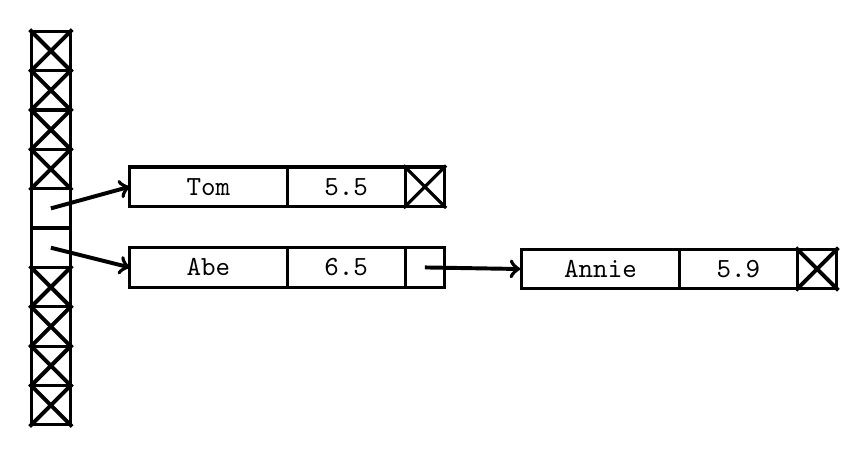
\begin{tikzpicture}
\draw[line width=0.05cm,black] (1.98,0.020000000000000018) to  (2.52,-0.52);
\draw[line width=0.05cm,black] (2.52,0.020000000000000018) to  (1.98,-0.52);
\draw[line width=0.05cm,black] (1.98,-0.48) to  (2.52,-1.02);
\draw[line width=0.05cm,black] (2.52,-0.48) to  (1.98,-1.02);
\draw[line width=0.05cm,black] (1.98,-0.98) to  (2.52,-1.52);
\draw[line width=0.05cm,black] (2.52,-0.98) to  (1.98,-1.52);
\draw[line width=0.05cm,black] (1.98,-1.48) to  (2.52,-2.02);
\draw[line width=0.05cm,black] (2.52,-1.48) to  (1.98,-2.02);

\draw (4.25, -1.975)
  node[draw, line width=0.04cm, , color=black,
       rounded corners=0cm, inner sep=0cm] {

\begin{minipage}[t][0.5cm]{2.0cm}
\mbox{}

\end{minipage}

};\draw (4.25, -1.975) node[color=black] {\texttt{Tom}};
\draw (6.0, -1.975)
  node[draw, line width=0.04cm, , color=black,
       rounded corners=0cm, inner sep=0cm] {

\begin{minipage}[t][0.5cm]{1.5cm}
\mbox{}

\end{minipage}

};\draw (6.0, -1.975) node[color=black] {\texttt{5.5}};
\draw (7.0, -1.975)
  node[draw, line width=0.04cm, , color=black,
       rounded corners=0cm, inner sep=0cm] {

\begin{minipage}[t][0.5cm]{0.5cm}
\mbox{}

\end{minipage}

};\draw[line width=0.05cm,black,->] (2.25,-2.25) to  (3.25,-1.9749999999999999);

\fill[black] (2.25, -2.25) circle (0);
\draw[black] (2.25, -2.25) circle (0.0);\draw[line width=0.04cm,black] (6.73,-1.705) to  (7.27,-2.245);
\draw[line width=0.04cm,black] (7.27,-1.705) to  (6.73,-2.245);

\draw (4.25, -3.0)
  node[draw, line width=0.04cm, , color=black,
       rounded corners=0cm, inner sep=0cm] {

\begin{minipage}[t][0.5cm]{2.0cm}
\mbox{}

\end{minipage}

};\draw (4.25, -3.0) node[color=black] {\texttt{Abe}};
\draw (6.0, -3.0)
  node[draw, line width=0.04cm, , color=black,
       rounded corners=0cm, inner sep=0cm] {

\begin{minipage}[t][0.5cm]{1.5cm}
\mbox{}

\end{minipage}

};\draw (6.0, -3.0) node[color=black] {\texttt{6.5}};
\draw (7.0, -3.0)
  node[draw, line width=0.04cm, , color=black,
       rounded corners=0cm, inner sep=0cm] {

\begin{minipage}[t][0.5cm]{0.5cm}
\mbox{}

\end{minipage}

};\draw[line width=0.05cm,black,->] (2.25,-2.75) to  (3.25,-3.0);

\fill[black] (2.25, -2.75) circle (0);
\draw[black] (2.25, -2.75) circle (0.0);
\draw (9.23, -3.02)
  node[draw, line width=0.04cm, , color=black,
       rounded corners=0cm, inner sep=0cm] {

\begin{minipage}[t][0.5cm]{2.0cm}
\mbox{}

\end{minipage}

};\draw (9.23, -3.02) node[color=black] {\texttt{Annie}};
\draw (10.98, -3.02)
  node[draw, line width=0.04cm, , color=black,
       rounded corners=0cm, inner sep=0cm] {

\begin{minipage}[t][0.5cm]{1.5cm}
\mbox{}

\end{minipage}

};\draw (10.98, -3.02) node[color=black] {\texttt{5.9}};
\draw (11.98, -3.02)
  node[draw, line width=0.04cm, , color=black,
       rounded corners=0cm, inner sep=0cm] {

\begin{minipage}[t][0.5cm]{0.5cm}
\mbox{}

\end{minipage}

};\draw[line width=0.05cm,black] (11.71,-2.75) to  (12.25,-3.29);
\draw[line width=0.05cm,black] (12.25,-2.75) to  (11.71,-3.29);
\draw[line width=0.05cm,black,->] (7.0,-3.0) to  (8.21,-3.0199999999999996);

\fill[black] (7.0, -3.0) circle (0);
\draw[black] (7.0, -3.0) circle (0.0);\draw[line width=0.05cm,black] (1.98,-2.98) to  (2.52,-3.52);
\draw[line width=0.05cm,black] (2.52,-2.98) to  (1.98,-3.52);
\draw[line width=0.05cm,black] (1.98,-3.4800000000000004) to  (2.52,-4.02);
\draw[line width=0.05cm,black] (2.52,-3.4800000000000004) to  (1.98,-4.02);
\draw[line width=0.05cm,black] (1.98,-3.9800000000000004) to  (2.52,-4.52);
\draw[line width=0.05cm,black] (2.52,-3.9800000000000004) to  (1.98,-4.52);
\draw[line width=0.05cm,black] (1.98,-4.48) to  (2.52,-5.02);
\draw[line width=0.05cm,black] (2.52,-4.48) to  (1.98,-5.02);

\draw (2.25, -0.25)
  node[draw, line width=0.04cm, , color=black,
       rounded corners=0cm, inner sep=0cm] {

\begin{minipage}[t][0.5cm]{0.5cm}
\mbox{}

\end{minipage}

};
\draw (2.25, -0.75)
  node[draw, line width=0.04cm, , color=black,
       rounded corners=0cm, inner sep=0cm] {

\begin{minipage}[t][0.5cm]{0.5cm}
\mbox{}

\end{minipage}

};
\draw (2.25, -1.25)
  node[draw, line width=0.04cm, , color=black,
       rounded corners=0cm, inner sep=0cm] {

\begin{minipage}[t][0.5cm]{0.5cm}
\mbox{}

\end{minipage}

};
\draw (2.25, -1.75)
  node[draw, line width=0.04cm, , color=black,
       rounded corners=0cm, inner sep=0cm] {

\begin{minipage}[t][0.5cm]{0.5cm}
\mbox{}

\end{minipage}

};
\draw (2.25, -2.25)
  node[draw, line width=0.04cm, , color=black,
       rounded corners=0cm, inner sep=0cm] {

\begin{minipage}[t][0.5cm]{0.5cm}
\mbox{}

\end{minipage}

};
\draw (2.25, -2.75)
  node[draw, line width=0.04cm, , color=black,
       rounded corners=0cm, inner sep=0cm] {

\begin{minipage}[t][0.5cm]{0.5cm}
\mbox{}

\end{minipage}

};
\draw (2.25, -3.25)
  node[draw, line width=0.04cm, , color=black,
       rounded corners=0cm, inner sep=0cm] {

\begin{minipage}[t][0.5cm]{0.5cm}
\mbox{}

\end{minipage}

};
\draw (2.25, -3.75)
  node[draw, line width=0.04cm, , color=black,
       rounded corners=0cm, inner sep=0cm] {

\begin{minipage}[t][0.5cm]{0.5cm}
\mbox{}

\end{minipage}

};
\draw (2.25, -4.25)
  node[draw, line width=0.04cm, , color=black,
       rounded corners=0cm, inner sep=0cm] {

\begin{minipage}[t][0.5cm]{0.5cm}
\mbox{}

\end{minipage}

};
\draw (2.25, -4.75)
  node[draw, line width=0.04cm, , color=black,
       rounded corners=0cm, inner sep=0cm] {

\begin{minipage}[t][0.5cm]{0.5cm}
\mbox{}

\end{minipage}

};
\end{tikzpicture}

\end{center}



to get


\begin{center}
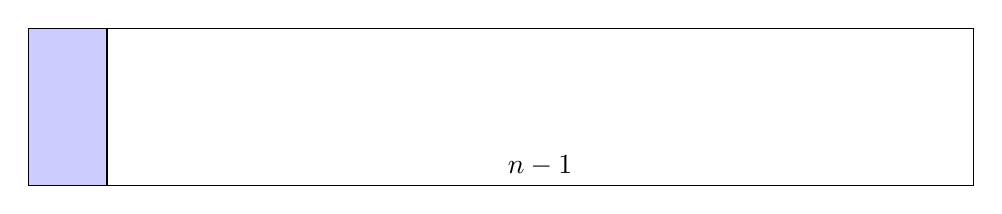
\begin{tikzpicture}

\draw (6.0, 1.0)
  node[draw, , , color=black,
       rounded corners=0cm, inner sep=0cm] {

\begin{minipage}[t][2cm]{12cm}
\mbox{}

\end{minipage}

};
\draw (0.5, 1.0)
  node[fill=blue!20!white,rounded corners=0cm,inner sep=0cm] {

\begin{minipage}[t][2cm]{1cm}
\mbox{}

\end{minipage}

};
\draw (0.5, 1.0)
  node[draw, , , color=black,
       rounded corners=0cm, inner sep=0cm] {

\begin{minipage}[t][2cm]{1cm}
\mbox{}

\end{minipage}

};
\draw (6.5, 0.25)
  node[draw=none, line width=0cm, , color=black,
       rounded corners=0cm, inner sep=0cm] {

\begin{minipage}[t][0.1cm]{0.1cm}
\mbox{}

\end{minipage}

};\draw (6.5, 0.25) node[color=black] {$n - 1$};
\end{tikzpicture}

\end{center}



I do it again, swapping \verb!0! with \verb!3! to get

\begin{center}
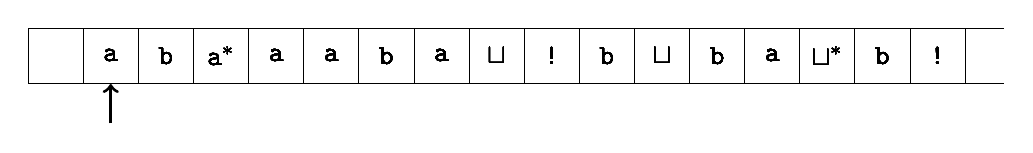
\begin{tikzpicture}

\draw (0.35, 0.35)
  node[draw, line width=0.01cm, , color=black,
       rounded corners=0cm, inner sep=0cm] {

\begin{minipage}[t][0.7cm]{0.7cm}
\mbox{}

\end{minipage}

};\draw (0.35, 0.35) node[color=black] {\texttt{\DOLLAR}};
\draw (1.0499999999999998, 0.35)
  node[draw, line width=0.01cm, , color=black,
       rounded corners=0cm, inner sep=0cm] {

\begin{minipage}[t][0.7cm]{0.7cm}
\mbox{}

\end{minipage}

};\draw (1.0499999999999998, 0.35) node[color=black] {\texttt{a}};
\draw (1.7499999999999998, 0.35)
  node[draw, line width=0.01cm, , color=black,
       rounded corners=0cm, inner sep=0cm] {

\begin{minipage}[t][0.7cm]{0.7cm}
\mbox{}

\end{minipage}

};\draw (1.7499999999999998, 0.35) node[color=black] {\texttt{b}};
\draw (2.4499999999999997, 0.35)
  node[draw, line width=0.01cm, , color=black,
       rounded corners=0cm, inner sep=0cm] {

\begin{minipage}[t][0.7cm]{0.7cm}
\mbox{}

\end{minipage}

};\draw (2.4499999999999997, 0.35) node[color=black] {\texttt{a$^*$}};
\draw (3.15, 0.35)
  node[draw, line width=0.01cm, , color=black,
       rounded corners=0cm, inner sep=0cm] {

\begin{minipage}[t][0.7cm]{0.7cm}
\mbox{}

\end{minipage}

};\draw (3.15, 0.35) node[color=black] {\texttt{a}};
\draw (3.85, 0.35)
  node[draw, line width=0.01cm, , color=black,
       rounded corners=0cm, inner sep=0cm] {

\begin{minipage}[t][0.7cm]{0.7cm}
\mbox{}

\end{minipage}

};\draw (3.85, 0.35) node[color=black] {\texttt{a}};
\draw (4.550000000000001, 0.35)
  node[draw, line width=0.01cm, , color=black,
       rounded corners=0cm, inner sep=0cm] {

\begin{minipage}[t][0.7cm]{0.7cm}
\mbox{}

\end{minipage}

};\draw (4.550000000000001, 0.35) node[color=black] {\texttt{b}};
\draw (5.25, 0.35)
  node[draw, line width=0.01cm, , color=black,
       rounded corners=0cm, inner sep=0cm] {

\begin{minipage}[t][0.7cm]{0.7cm}
\mbox{}

\end{minipage}

};\draw (5.25, 0.35) node[color=black] {\texttt{a}};
\draw (5.950000000000001, 0.35)
  node[draw, line width=0.01cm, , color=black,
       rounded corners=0cm, inner sep=0cm] {

\begin{minipage}[t][0.7cm]{0.7cm}
\mbox{}

\end{minipage}

};\draw (5.950000000000001, 0.35) node[color=black] {\texttt{$\sqcup$}};
\draw (6.65, 0.35)
  node[draw, line width=0.01cm, , color=black,
       rounded corners=0cm, inner sep=0cm] {

\begin{minipage}[t][0.7cm]{0.7cm}
\mbox{}

\end{minipage}

};\draw (6.65, 0.35) node[color=black] {\texttt{!}};
\draw (7.350000000000001, 0.35)
  node[draw, line width=0.01cm, , color=black,
       rounded corners=0cm, inner sep=0cm] {

\begin{minipage}[t][0.7cm]{0.7cm}
\mbox{}

\end{minipage}

};\draw (7.350000000000001, 0.35) node[color=black] {\texttt{b}};
\draw (8.05, 0.35)
  node[draw, line width=0.01cm, , color=black,
       rounded corners=0cm, inner sep=0cm] {

\begin{minipage}[t][0.7cm]{0.7cm}
\mbox{}

\end{minipage}

};\draw (8.05, 0.35) node[color=black] {\texttt{$\sqcup$}};
\draw (8.75, 0.35)
  node[draw, line width=0.01cm, , color=black,
       rounded corners=0cm, inner sep=0cm] {

\begin{minipage}[t][0.7cm]{0.7cm}
\mbox{}

\end{minipage}

};\draw (8.75, 0.35) node[color=black] {\texttt{b}};
\draw (9.45, 0.35)
  node[draw, line width=0.01cm, , color=black,
       rounded corners=0cm, inner sep=0cm] {

\begin{minipage}[t][0.7cm]{0.7cm}
\mbox{}

\end{minipage}

};\draw (9.45, 0.35) node[color=black] {\texttt{a}};
\draw (10.149999999999999, 0.35)
  node[draw, line width=0.01cm, , color=black,
       rounded corners=0cm, inner sep=0cm] {

\begin{minipage}[t][0.7cm]{0.7cm}
\mbox{}

\end{minipage}

};\draw (10.149999999999999, 0.35) node[color=black] {\texttt{$\sqcup^*$}};
\draw (10.849999999999998, 0.35)
  node[draw, line width=0.01cm, , color=black,
       rounded corners=0cm, inner sep=0cm] {

\begin{minipage}[t][0.7cm]{0.7cm}
\mbox{}

\end{minipage}

};\draw (10.849999999999998, 0.35) node[color=black] {\texttt{b}};
\draw (11.549999999999997, 0.35)
  node[draw, line width=0.01cm, , color=black,
       rounded corners=0cm, inner sep=0cm] {

\begin{minipage}[t][0.7cm]{0.7cm}
\mbox{}

\end{minipage}

};\draw (11.549999999999997, 0.35) node[color=black] {\texttt{!}};
\draw (0.35, 0.35)
  node[draw, line width=0.01cm, , color=black,
       rounded corners=0cm, inner sep=0cm] {

\begin{minipage}[t][0.7cm]{0.7cm}
\mbox{}

\end{minipage}

};\draw (0.35, 0.35) node[color=black] {\texttt{\DOLLAR}};
\draw (1.0499999999999998, 0.35)
  node[draw, line width=0.01cm, , color=black,
       rounded corners=0cm, inner sep=0cm] {

\begin{minipage}[t][0.7cm]{0.7cm}
\mbox{}

\end{minipage}

};\draw (1.0499999999999998, 0.35) node[color=black] {\texttt{a}};
\draw (1.7499999999999998, 0.35)
  node[draw, line width=0.01cm, , color=black,
       rounded corners=0cm, inner sep=0cm] {

\begin{minipage}[t][0.7cm]{0.7cm}
\mbox{}

\end{minipage}

};\draw (1.7499999999999998, 0.35) node[color=black] {\texttt{b}};
\draw (2.4499999999999997, 0.35)
  node[draw, line width=0.01cm, , color=black,
       rounded corners=0cm, inner sep=0cm] {

\begin{minipage}[t][0.7cm]{0.7cm}
\mbox{}

\end{minipage}

};\draw (2.4499999999999997, 0.35) node[color=black] {\texttt{a$^*$}};
\draw (3.15, 0.35)
  node[draw, line width=0.01cm, , color=black,
       rounded corners=0cm, inner sep=0cm] {

\begin{minipage}[t][0.7cm]{0.7cm}
\mbox{}

\end{minipage}

};\draw (3.15, 0.35) node[color=black] {\texttt{a}};
\draw (3.85, 0.35)
  node[draw, line width=0.01cm, , color=black,
       rounded corners=0cm, inner sep=0cm] {

\begin{minipage}[t][0.7cm]{0.7cm}
\mbox{}

\end{minipage}

};\draw (3.85, 0.35) node[color=black] {\texttt{a}};
\draw (4.550000000000001, 0.35)
  node[draw, line width=0.01cm, , color=black,
       rounded corners=0cm, inner sep=0cm] {

\begin{minipage}[t][0.7cm]{0.7cm}
\mbox{}

\end{minipage}

};\draw (4.550000000000001, 0.35) node[color=black] {\texttt{b}};
\draw (5.25, 0.35)
  node[draw, line width=0.01cm, , color=black,
       rounded corners=0cm, inner sep=0cm] {

\begin{minipage}[t][0.7cm]{0.7cm}
\mbox{}

\end{minipage}

};\draw (5.25, 0.35) node[color=black] {\texttt{a}};
\draw (5.950000000000001, 0.35)
  node[draw, line width=0.01cm, , color=black,
       rounded corners=0cm, inner sep=0cm] {

\begin{minipage}[t][0.7cm]{0.7cm}
\mbox{}

\end{minipage}

};\draw (5.950000000000001, 0.35) node[color=black] {\texttt{$\sqcup$}};
\draw (6.65, 0.35)
  node[draw, line width=0.01cm, , color=black,
       rounded corners=0cm, inner sep=0cm] {

\begin{minipage}[t][0.7cm]{0.7cm}
\mbox{}

\end{minipage}

};\draw (6.65, 0.35) node[color=black] {\texttt{!}};
\draw (7.350000000000001, 0.35)
  node[draw, line width=0.01cm, , color=black,
       rounded corners=0cm, inner sep=0cm] {

\begin{minipage}[t][0.7cm]{0.7cm}
\mbox{}

\end{minipage}

};\draw (7.350000000000001, 0.35) node[color=black] {\texttt{b}};
\draw (8.05, 0.35)
  node[draw, line width=0.01cm, , color=black,
       rounded corners=0cm, inner sep=0cm] {

\begin{minipage}[t][0.7cm]{0.7cm}
\mbox{}

\end{minipage}

};\draw (8.05, 0.35) node[color=black] {\texttt{$\sqcup$}};
\draw (8.75, 0.35)
  node[draw, line width=0.01cm, , color=black,
       rounded corners=0cm, inner sep=0cm] {

\begin{minipage}[t][0.7cm]{0.7cm}
\mbox{}

\end{minipage}

};\draw (8.75, 0.35) node[color=black] {\texttt{b}};
\draw (9.45, 0.35)
  node[draw, line width=0.01cm, , color=black,
       rounded corners=0cm, inner sep=0cm] {

\begin{minipage}[t][0.7cm]{0.7cm}
\mbox{}

\end{minipage}

};\draw (9.45, 0.35) node[color=black] {\texttt{a}};
\draw (10.149999999999999, 0.35)
  node[draw, line width=0.01cm, , color=black,
       rounded corners=0cm, inner sep=0cm] {

\begin{minipage}[t][0.7cm]{0.7cm}
\mbox{}

\end{minipage}

};\draw (10.149999999999999, 0.35) node[color=black] {\texttt{$\sqcup^*$}};
\draw (10.849999999999998, 0.35)
  node[draw, line width=0.01cm, , color=black,
       rounded corners=0cm, inner sep=0cm] {

\begin{minipage}[t][0.7cm]{0.7cm}
\mbox{}

\end{minipage}

};\draw (10.849999999999998, 0.35) node[color=black] {\texttt{b}};
\draw (11.549999999999997, 0.35)
  node[draw, line width=0.01cm, , color=black,
       rounded corners=0cm, inner sep=0cm] {

\begin{minipage}[t][0.7cm]{0.7cm}
\mbox{}

\end{minipage}

};\draw (11.549999999999997, 0.35) node[color=black] {\texttt{!}};
\draw (0.35, 0.35)
  node[draw, line width=0.01cm, , color=black,
       rounded corners=0cm, inner sep=0cm] {

\begin{minipage}[t][0.7cm]{0.7cm}
\mbox{}

\end{minipage}

};\draw (0.35, 0.35) node[color=black] {\texttt{\DOLLAR}};
\draw (1.0499999999999998, 0.35)
  node[draw, line width=0.01cm, , color=black,
       rounded corners=0cm, inner sep=0cm] {

\begin{minipage}[t][0.7cm]{0.7cm}
\mbox{}

\end{minipage}

};\draw (1.0499999999999998, 0.35) node[color=black] {\texttt{a}};
\draw (1.7499999999999998, 0.35)
  node[draw, line width=0.01cm, , color=black,
       rounded corners=0cm, inner sep=0cm] {

\begin{minipage}[t][0.7cm]{0.7cm}
\mbox{}

\end{minipage}

};\draw (1.7499999999999998, 0.35) node[color=black] {\texttt{b}};
\draw (2.4499999999999997, 0.35)
  node[draw, line width=0.01cm, , color=black,
       rounded corners=0cm, inner sep=0cm] {

\begin{minipage}[t][0.7cm]{0.7cm}
\mbox{}

\end{minipage}

};\draw (2.4499999999999997, 0.35) node[color=black] {\texttt{a$^*$}};
\draw (3.15, 0.35)
  node[draw, line width=0.01cm, , color=black,
       rounded corners=0cm, inner sep=0cm] {

\begin{minipage}[t][0.7cm]{0.7cm}
\mbox{}

\end{minipage}

};\draw (3.15, 0.35) node[color=black] {\texttt{a}};
\draw (3.85, 0.35)
  node[draw, line width=0.01cm, , color=black,
       rounded corners=0cm, inner sep=0cm] {

\begin{minipage}[t][0.7cm]{0.7cm}
\mbox{}

\end{minipage}

};\draw (3.85, 0.35) node[color=black] {\texttt{a}};
\draw (4.550000000000001, 0.35)
  node[draw, line width=0.01cm, , color=black,
       rounded corners=0cm, inner sep=0cm] {

\begin{minipage}[t][0.7cm]{0.7cm}
\mbox{}

\end{minipage}

};\draw (4.550000000000001, 0.35) node[color=black] {\texttt{b}};
\draw (5.25, 0.35)
  node[draw, line width=0.01cm, , color=black,
       rounded corners=0cm, inner sep=0cm] {

\begin{minipage}[t][0.7cm]{0.7cm}
\mbox{}

\end{minipage}

};\draw (5.25, 0.35) node[color=black] {\texttt{a}};
\draw (5.950000000000001, 0.35)
  node[draw, line width=0.01cm, , color=black,
       rounded corners=0cm, inner sep=0cm] {

\begin{minipage}[t][0.7cm]{0.7cm}
\mbox{}

\end{minipage}

};\draw (5.950000000000001, 0.35) node[color=black] {\texttt{$\sqcup$}};
\draw (6.65, 0.35)
  node[draw, line width=0.01cm, , color=black,
       rounded corners=0cm, inner sep=0cm] {

\begin{minipage}[t][0.7cm]{0.7cm}
\mbox{}

\end{minipage}

};\draw (6.65, 0.35) node[color=black] {\texttt{!}};
\draw (7.350000000000001, 0.35)
  node[draw, line width=0.01cm, , color=black,
       rounded corners=0cm, inner sep=0cm] {

\begin{minipage}[t][0.7cm]{0.7cm}
\mbox{}

\end{minipage}

};\draw (7.350000000000001, 0.35) node[color=black] {\texttt{b}};
\draw (8.05, 0.35)
  node[draw, line width=0.01cm, , color=black,
       rounded corners=0cm, inner sep=0cm] {

\begin{minipage}[t][0.7cm]{0.7cm}
\mbox{}

\end{minipage}

};\draw (8.05, 0.35) node[color=black] {\texttt{$\sqcup$}};
\draw (8.75, 0.35)
  node[draw, line width=0.01cm, , color=black,
       rounded corners=0cm, inner sep=0cm] {

\begin{minipage}[t][0.7cm]{0.7cm}
\mbox{}

\end{minipage}

};\draw (8.75, 0.35) node[color=black] {\texttt{b}};
\draw (9.45, 0.35)
  node[draw, line width=0.01cm, , color=black,
       rounded corners=0cm, inner sep=0cm] {

\begin{minipage}[t][0.7cm]{0.7cm}
\mbox{}

\end{minipage}

};\draw (9.45, 0.35) node[color=black] {\texttt{a}};
\draw (10.149999999999999, 0.35)
  node[draw, line width=0.01cm, , color=black,
       rounded corners=0cm, inner sep=0cm] {

\begin{minipage}[t][0.7cm]{0.7cm}
\mbox{}

\end{minipage}

};\draw (10.149999999999999, 0.35) node[color=black] {\texttt{$\sqcup^*$}};
\draw (10.849999999999998, 0.35)
  node[draw, line width=0.01cm, , color=black,
       rounded corners=0cm, inner sep=0cm] {

\begin{minipage}[t][0.7cm]{0.7cm}
\mbox{}

\end{minipage}

};\draw (10.849999999999998, 0.35) node[color=black] {\texttt{b}};
\draw (11.549999999999997, 0.35)
  node[draw, line width=0.01cm, , color=black,
       rounded corners=0cm, inner sep=0cm] {

\begin{minipage}[t][0.7cm]{0.7cm}
\mbox{}

\end{minipage}

};\draw (11.549999999999997, 0.35) node[color=black] {\texttt{!}};
\draw (0.35, 0.35)
  node[draw, line width=0.01cm, , color=black,
       rounded corners=0cm, inner sep=0cm] {

\begin{minipage}[t][0.7cm]{0.7cm}
\mbox{}

\end{minipage}

};\draw (0.35, 0.35) node[color=black] {\texttt{\DOLLAR}};
\draw (1.0499999999999998, 0.35)
  node[draw, line width=0.01cm, , color=black,
       rounded corners=0cm, inner sep=0cm] {

\begin{minipage}[t][0.7cm]{0.7cm}
\mbox{}

\end{minipage}

};\draw (1.0499999999999998, 0.35) node[color=black] {\texttt{a}};
\draw (1.7499999999999998, 0.35)
  node[draw, line width=0.01cm, , color=black,
       rounded corners=0cm, inner sep=0cm] {

\begin{minipage}[t][0.7cm]{0.7cm}
\mbox{}

\end{minipage}

};\draw (1.7499999999999998, 0.35) node[color=black] {\texttt{b}};
\draw (2.4499999999999997, 0.35)
  node[draw, line width=0.01cm, , color=black,
       rounded corners=0cm, inner sep=0cm] {

\begin{minipage}[t][0.7cm]{0.7cm}
\mbox{}

\end{minipage}

};\draw (2.4499999999999997, 0.35) node[color=black] {\texttt{a$^*$}};
\draw (3.15, 0.35)
  node[draw, line width=0.01cm, , color=black,
       rounded corners=0cm, inner sep=0cm] {

\begin{minipage}[t][0.7cm]{0.7cm}
\mbox{}

\end{minipage}

};\draw (3.15, 0.35) node[color=black] {\texttt{a}};
\draw (3.85, 0.35)
  node[draw, line width=0.01cm, , color=black,
       rounded corners=0cm, inner sep=0cm] {

\begin{minipage}[t][0.7cm]{0.7cm}
\mbox{}

\end{minipage}

};\draw (3.85, 0.35) node[color=black] {\texttt{a}};
\draw (4.550000000000001, 0.35)
  node[draw, line width=0.01cm, , color=black,
       rounded corners=0cm, inner sep=0cm] {

\begin{minipage}[t][0.7cm]{0.7cm}
\mbox{}

\end{minipage}

};\draw (4.550000000000001, 0.35) node[color=black] {\texttt{b}};
\draw (5.25, 0.35)
  node[draw, line width=0.01cm, , color=black,
       rounded corners=0cm, inner sep=0cm] {

\begin{minipage}[t][0.7cm]{0.7cm}
\mbox{}

\end{minipage}

};\draw (5.25, 0.35) node[color=black] {\texttt{a}};
\draw (5.950000000000001, 0.35)
  node[draw, line width=0.01cm, , color=black,
       rounded corners=0cm, inner sep=0cm] {

\begin{minipage}[t][0.7cm]{0.7cm}
\mbox{}

\end{minipage}

};\draw (5.950000000000001, 0.35) node[color=black] {\texttt{$\sqcup$}};
\draw (6.65, 0.35)
  node[draw, line width=0.01cm, , color=black,
       rounded corners=0cm, inner sep=0cm] {

\begin{minipage}[t][0.7cm]{0.7cm}
\mbox{}

\end{minipage}

};\draw (6.65, 0.35) node[color=black] {\texttt{!}};
\draw (7.350000000000001, 0.35)
  node[draw, line width=0.01cm, , color=black,
       rounded corners=0cm, inner sep=0cm] {

\begin{minipage}[t][0.7cm]{0.7cm}
\mbox{}

\end{minipage}

};\draw (7.350000000000001, 0.35) node[color=black] {\texttt{b}};
\draw (8.05, 0.35)
  node[draw, line width=0.01cm, , color=black,
       rounded corners=0cm, inner sep=0cm] {

\begin{minipage}[t][0.7cm]{0.7cm}
\mbox{}

\end{minipage}

};\draw (8.05, 0.35) node[color=black] {\texttt{$\sqcup$}};
\draw (8.75, 0.35)
  node[draw, line width=0.01cm, , color=black,
       rounded corners=0cm, inner sep=0cm] {

\begin{minipage}[t][0.7cm]{0.7cm}
\mbox{}

\end{minipage}

};\draw (8.75, 0.35) node[color=black] {\texttt{b}};
\draw (9.45, 0.35)
  node[draw, line width=0.01cm, , color=black,
       rounded corners=0cm, inner sep=0cm] {

\begin{minipage}[t][0.7cm]{0.7cm}
\mbox{}

\end{minipage}

};\draw (9.45, 0.35) node[color=black] {\texttt{a}};
\draw (10.149999999999999, 0.35)
  node[draw, line width=0.01cm, , color=black,
       rounded corners=0cm, inner sep=0cm] {

\begin{minipage}[t][0.7cm]{0.7cm}
\mbox{}

\end{minipage}

};\draw (10.149999999999999, 0.35) node[color=black] {\texttt{$\sqcup^*$}};
\draw (10.849999999999998, 0.35)
  node[draw, line width=0.01cm, , color=black,
       rounded corners=0cm, inner sep=0cm] {

\begin{minipage}[t][0.7cm]{0.7cm}
\mbox{}

\end{minipage}

};\draw (10.849999999999998, 0.35) node[color=black] {\texttt{b}};
\draw (11.549999999999997, 0.35)
  node[draw, line width=0.01cm, , color=black,
       rounded corners=0cm, inner sep=0cm] {

\begin{minipage}[t][0.7cm]{0.7cm}
\mbox{}

\end{minipage}

};\draw (11.549999999999997, 0.35) node[color=black] {\texttt{!}};
\draw (0.35, 0.35)
  node[draw, line width=0.01cm, , color=black,
       rounded corners=0cm, inner sep=0cm] {

\begin{minipage}[t][0.7cm]{0.7cm}
\mbox{}

\end{minipage}

};\draw (0.35, 0.35) node[color=black] {\texttt{\DOLLAR}};
\draw (1.0499999999999998, 0.35)
  node[draw, line width=0.01cm, , color=black,
       rounded corners=0cm, inner sep=0cm] {

\begin{minipage}[t][0.7cm]{0.7cm}
\mbox{}

\end{minipage}

};\draw (1.0499999999999998, 0.35) node[color=black] {\texttt{a}};
\draw (1.7499999999999998, 0.35)
  node[draw, line width=0.01cm, , color=black,
       rounded corners=0cm, inner sep=0cm] {

\begin{minipage}[t][0.7cm]{0.7cm}
\mbox{}

\end{minipage}

};\draw (1.7499999999999998, 0.35) node[color=black] {\texttt{b}};
\draw (2.4499999999999997, 0.35)
  node[draw, line width=0.01cm, , color=black,
       rounded corners=0cm, inner sep=0cm] {

\begin{minipage}[t][0.7cm]{0.7cm}
\mbox{}

\end{minipage}

};\draw (2.4499999999999997, 0.35) node[color=black] {\texttt{a$^*$}};
\draw (3.15, 0.35)
  node[draw, line width=0.01cm, , color=black,
       rounded corners=0cm, inner sep=0cm] {

\begin{minipage}[t][0.7cm]{0.7cm}
\mbox{}

\end{minipage}

};\draw (3.15, 0.35) node[color=black] {\texttt{a}};
\draw (3.85, 0.35)
  node[draw, line width=0.01cm, , color=black,
       rounded corners=0cm, inner sep=0cm] {

\begin{minipage}[t][0.7cm]{0.7cm}
\mbox{}

\end{minipage}

};\draw (3.85, 0.35) node[color=black] {\texttt{a}};
\draw (4.550000000000001, 0.35)
  node[draw, line width=0.01cm, , color=black,
       rounded corners=0cm, inner sep=0cm] {

\begin{minipage}[t][0.7cm]{0.7cm}
\mbox{}

\end{minipage}

};\draw (4.550000000000001, 0.35) node[color=black] {\texttt{b}};
\draw (5.25, 0.35)
  node[draw, line width=0.01cm, , color=black,
       rounded corners=0cm, inner sep=0cm] {

\begin{minipage}[t][0.7cm]{0.7cm}
\mbox{}

\end{minipage}

};\draw (5.25, 0.35) node[color=black] {\texttt{a}};
\draw (5.950000000000001, 0.35)
  node[draw, line width=0.01cm, , color=black,
       rounded corners=0cm, inner sep=0cm] {

\begin{minipage}[t][0.7cm]{0.7cm}
\mbox{}

\end{minipage}

};\draw (5.950000000000001, 0.35) node[color=black] {\texttt{$\sqcup$}};
\draw (6.65, 0.35)
  node[draw, line width=0.01cm, , color=black,
       rounded corners=0cm, inner sep=0cm] {

\begin{minipage}[t][0.7cm]{0.7cm}
\mbox{}

\end{minipage}

};\draw (6.65, 0.35) node[color=black] {\texttt{!}};
\draw (7.350000000000001, 0.35)
  node[draw, line width=0.01cm, , color=black,
       rounded corners=0cm, inner sep=0cm] {

\begin{minipage}[t][0.7cm]{0.7cm}
\mbox{}

\end{minipage}

};\draw (7.350000000000001, 0.35) node[color=black] {\texttt{b}};
\draw (8.05, 0.35)
  node[draw, line width=0.01cm, , color=black,
       rounded corners=0cm, inner sep=0cm] {

\begin{minipage}[t][0.7cm]{0.7cm}
\mbox{}

\end{minipage}

};\draw (8.05, 0.35) node[color=black] {\texttt{$\sqcup$}};
\draw (8.75, 0.35)
  node[draw, line width=0.01cm, , color=black,
       rounded corners=0cm, inner sep=0cm] {

\begin{minipage}[t][0.7cm]{0.7cm}
\mbox{}

\end{minipage}

};\draw (8.75, 0.35) node[color=black] {\texttt{b}};
\draw (9.45, 0.35)
  node[draw, line width=0.01cm, , color=black,
       rounded corners=0cm, inner sep=0cm] {

\begin{minipage}[t][0.7cm]{0.7cm}
\mbox{}

\end{minipage}

};\draw (9.45, 0.35) node[color=black] {\texttt{a}};
\draw (10.149999999999999, 0.35)
  node[draw, line width=0.01cm, , color=black,
       rounded corners=0cm, inner sep=0cm] {

\begin{minipage}[t][0.7cm]{0.7cm}
\mbox{}

\end{minipage}

};\draw (10.149999999999999, 0.35) node[color=black] {\texttt{$\sqcup^*$}};
\draw (10.849999999999998, 0.35)
  node[draw, line width=0.01cm, , color=black,
       rounded corners=0cm, inner sep=0cm] {

\begin{minipage}[t][0.7cm]{0.7cm}
\mbox{}

\end{minipage}

};\draw (10.849999999999998, 0.35) node[color=black] {\texttt{b}};
\draw (11.549999999999997, 0.35)
  node[draw, line width=0.01cm, , color=black,
       rounded corners=0cm, inner sep=0cm] {

\begin{minipage}[t][0.7cm]{0.7cm}
\mbox{}

\end{minipage}

};\draw (11.549999999999997, 0.35) node[color=black] {\texttt{!}};
\draw (0.35, 0.35)
  node[draw, line width=0.01cm, , color=black,
       rounded corners=0cm, inner sep=0cm] {

\begin{minipage}[t][0.7cm]{0.7cm}
\mbox{}

\end{minipage}

};\draw (0.35, 0.35) node[color=black] {\texttt{\DOLLAR}};
\draw (1.0499999999999998, 0.35)
  node[draw, line width=0.01cm, , color=black,
       rounded corners=0cm, inner sep=0cm] {

\begin{minipage}[t][0.7cm]{0.7cm}
\mbox{}

\end{minipage}

};\draw (1.0499999999999998, 0.35) node[color=black] {\texttt{a}};
\draw (1.7499999999999998, 0.35)
  node[draw, line width=0.01cm, , color=black,
       rounded corners=0cm, inner sep=0cm] {

\begin{minipage}[t][0.7cm]{0.7cm}
\mbox{}

\end{minipage}

};\draw (1.7499999999999998, 0.35) node[color=black] {\texttt{b}};
\draw (2.4499999999999997, 0.35)
  node[draw, line width=0.01cm, , color=black,
       rounded corners=0cm, inner sep=0cm] {

\begin{minipage}[t][0.7cm]{0.7cm}
\mbox{}

\end{minipage}

};\draw (2.4499999999999997, 0.35) node[color=black] {\texttt{a$^*$}};
\draw (3.15, 0.35)
  node[draw, line width=0.01cm, , color=black,
       rounded corners=0cm, inner sep=0cm] {

\begin{minipage}[t][0.7cm]{0.7cm}
\mbox{}

\end{minipage}

};\draw (3.15, 0.35) node[color=black] {\texttt{a}};
\draw (3.85, 0.35)
  node[draw, line width=0.01cm, , color=black,
       rounded corners=0cm, inner sep=0cm] {

\begin{minipage}[t][0.7cm]{0.7cm}
\mbox{}

\end{minipage}

};\draw (3.85, 0.35) node[color=black] {\texttt{a}};
\draw (4.550000000000001, 0.35)
  node[draw, line width=0.01cm, , color=black,
       rounded corners=0cm, inner sep=0cm] {

\begin{minipage}[t][0.7cm]{0.7cm}
\mbox{}

\end{minipage}

};\draw (4.550000000000001, 0.35) node[color=black] {\texttt{b}};
\draw (5.25, 0.35)
  node[draw, line width=0.01cm, , color=black,
       rounded corners=0cm, inner sep=0cm] {

\begin{minipage}[t][0.7cm]{0.7cm}
\mbox{}

\end{minipage}

};\draw (5.25, 0.35) node[color=black] {\texttt{a}};
\draw (5.950000000000001, 0.35)
  node[draw, line width=0.01cm, , color=black,
       rounded corners=0cm, inner sep=0cm] {

\begin{minipage}[t][0.7cm]{0.7cm}
\mbox{}

\end{minipage}

};\draw (5.950000000000001, 0.35) node[color=black] {\texttt{$\sqcup$}};
\draw (6.65, 0.35)
  node[draw, line width=0.01cm, , color=black,
       rounded corners=0cm, inner sep=0cm] {

\begin{minipage}[t][0.7cm]{0.7cm}
\mbox{}

\end{minipage}

};\draw (6.65, 0.35) node[color=black] {\texttt{!}};
\draw (7.350000000000001, 0.35)
  node[draw, line width=0.01cm, , color=black,
       rounded corners=0cm, inner sep=0cm] {

\begin{minipage}[t][0.7cm]{0.7cm}
\mbox{}

\end{minipage}

};\draw (7.350000000000001, 0.35) node[color=black] {\texttt{b}};
\draw (8.05, 0.35)
  node[draw, line width=0.01cm, , color=black,
       rounded corners=0cm, inner sep=0cm] {

\begin{minipage}[t][0.7cm]{0.7cm}
\mbox{}

\end{minipage}

};\draw (8.05, 0.35) node[color=black] {\texttt{$\sqcup$}};
\draw (8.75, 0.35)
  node[draw, line width=0.01cm, , color=black,
       rounded corners=0cm, inner sep=0cm] {

\begin{minipage}[t][0.7cm]{0.7cm}
\mbox{}

\end{minipage}

};\draw (8.75, 0.35) node[color=black] {\texttt{b}};
\draw (9.45, 0.35)
  node[draw, line width=0.01cm, , color=black,
       rounded corners=0cm, inner sep=0cm] {

\begin{minipage}[t][0.7cm]{0.7cm}
\mbox{}

\end{minipage}

};\draw (9.45, 0.35) node[color=black] {\texttt{a}};
\draw (10.149999999999999, 0.35)
  node[draw, line width=0.01cm, , color=black,
       rounded corners=0cm, inner sep=0cm] {

\begin{minipage}[t][0.7cm]{0.7cm}
\mbox{}

\end{minipage}

};\draw (10.149999999999999, 0.35) node[color=black] {\texttt{$\sqcup^*$}};
\draw (10.849999999999998, 0.35)
  node[draw, line width=0.01cm, , color=black,
       rounded corners=0cm, inner sep=0cm] {

\begin{minipage}[t][0.7cm]{0.7cm}
\mbox{}

\end{minipage}

};\draw (10.849999999999998, 0.35) node[color=black] {\texttt{b}};
\draw (11.549999999999997, 0.35)
  node[draw, line width=0.01cm, , color=black,
       rounded corners=0cm, inner sep=0cm] {

\begin{minipage}[t][0.7cm]{0.7cm}
\mbox{}

\end{minipage}

};\draw (11.549999999999997, 0.35) node[color=black] {\texttt{!}};
\draw (0.35, 0.35)
  node[draw, line width=0.01cm, , color=black,
       rounded corners=0cm, inner sep=0cm] {

\begin{minipage}[t][0.7cm]{0.7cm}
\mbox{}

\end{minipage}

};\draw (0.35, 0.35) node[color=black] {\texttt{\DOLLAR}};
\draw (1.0499999999999998, 0.35)
  node[draw, line width=0.01cm, , color=black,
       rounded corners=0cm, inner sep=0cm] {

\begin{minipage}[t][0.7cm]{0.7cm}
\mbox{}

\end{minipage}

};\draw (1.0499999999999998, 0.35) node[color=black] {\texttt{a}};
\draw (1.7499999999999998, 0.35)
  node[draw, line width=0.01cm, , color=black,
       rounded corners=0cm, inner sep=0cm] {

\begin{minipage}[t][0.7cm]{0.7cm}
\mbox{}

\end{minipage}

};\draw (1.7499999999999998, 0.35) node[color=black] {\texttt{b}};
\draw (2.4499999999999997, 0.35)
  node[draw, line width=0.01cm, , color=black,
       rounded corners=0cm, inner sep=0cm] {

\begin{minipage}[t][0.7cm]{0.7cm}
\mbox{}

\end{minipage}

};\draw (2.4499999999999997, 0.35) node[color=black] {\texttt{a$^*$}};
\draw (3.15, 0.35)
  node[draw, line width=0.01cm, , color=black,
       rounded corners=0cm, inner sep=0cm] {

\begin{minipage}[t][0.7cm]{0.7cm}
\mbox{}

\end{minipage}

};\draw (3.15, 0.35) node[color=black] {\texttt{a}};
\draw (3.85, 0.35)
  node[draw, line width=0.01cm, , color=black,
       rounded corners=0cm, inner sep=0cm] {

\begin{minipage}[t][0.7cm]{0.7cm}
\mbox{}

\end{minipage}

};\draw (3.85, 0.35) node[color=black] {\texttt{a}};
\draw (4.550000000000001, 0.35)
  node[draw, line width=0.01cm, , color=black,
       rounded corners=0cm, inner sep=0cm] {

\begin{minipage}[t][0.7cm]{0.7cm}
\mbox{}

\end{minipage}

};\draw (4.550000000000001, 0.35) node[color=black] {\texttt{b}};
\draw (5.25, 0.35)
  node[draw, line width=0.01cm, , color=black,
       rounded corners=0cm, inner sep=0cm] {

\begin{minipage}[t][0.7cm]{0.7cm}
\mbox{}

\end{minipage}

};\draw (5.25, 0.35) node[color=black] {\texttt{a}};
\draw (5.950000000000001, 0.35)
  node[draw, line width=0.01cm, , color=black,
       rounded corners=0cm, inner sep=0cm] {

\begin{minipage}[t][0.7cm]{0.7cm}
\mbox{}

\end{minipage}

};\draw (5.950000000000001, 0.35) node[color=black] {\texttt{$\sqcup$}};
\draw (6.65, 0.35)
  node[draw, line width=0.01cm, , color=black,
       rounded corners=0cm, inner sep=0cm] {

\begin{minipage}[t][0.7cm]{0.7cm}
\mbox{}

\end{minipage}

};\draw (6.65, 0.35) node[color=black] {\texttt{!}};
\draw (7.350000000000001, 0.35)
  node[draw, line width=0.01cm, , color=black,
       rounded corners=0cm, inner sep=0cm] {

\begin{minipage}[t][0.7cm]{0.7cm}
\mbox{}

\end{minipage}

};\draw (7.350000000000001, 0.35) node[color=black] {\texttt{b}};
\draw (8.05, 0.35)
  node[draw, line width=0.01cm, , color=black,
       rounded corners=0cm, inner sep=0cm] {

\begin{minipage}[t][0.7cm]{0.7cm}
\mbox{}

\end{minipage}

};\draw (8.05, 0.35) node[color=black] {\texttt{$\sqcup$}};
\draw (8.75, 0.35)
  node[draw, line width=0.01cm, , color=black,
       rounded corners=0cm, inner sep=0cm] {

\begin{minipage}[t][0.7cm]{0.7cm}
\mbox{}

\end{minipage}

};\draw (8.75, 0.35) node[color=black] {\texttt{b}};
\draw (9.45, 0.35)
  node[draw, line width=0.01cm, , color=black,
       rounded corners=0cm, inner sep=0cm] {

\begin{minipage}[t][0.7cm]{0.7cm}
\mbox{}

\end{minipage}

};\draw (9.45, 0.35) node[color=black] {\texttt{a}};
\draw (10.149999999999999, 0.35)
  node[draw, line width=0.01cm, , color=black,
       rounded corners=0cm, inner sep=0cm] {

\begin{minipage}[t][0.7cm]{0.7cm}
\mbox{}

\end{minipage}

};\draw (10.149999999999999, 0.35) node[color=black] {\texttt{$\sqcup^*$}};
\draw (10.849999999999998, 0.35)
  node[draw, line width=0.01cm, , color=black,
       rounded corners=0cm, inner sep=0cm] {

\begin{minipage}[t][0.7cm]{0.7cm}
\mbox{}

\end{minipage}

};\draw (10.849999999999998, 0.35) node[color=black] {\texttt{b}};
\draw (11.549999999999997, 0.35)
  node[draw, line width=0.01cm, , color=black,
       rounded corners=0cm, inner sep=0cm] {

\begin{minipage}[t][0.7cm]{0.7cm}
\mbox{}

\end{minipage}

};\draw (11.549999999999997, 0.35) node[color=black] {\texttt{!}};
\draw (0.35, 0.35)
  node[draw, line width=0.01cm, , color=black,
       rounded corners=0cm, inner sep=0cm] {

\begin{minipage}[t][0.7cm]{0.7cm}
\mbox{}

\end{minipage}

};\draw (0.35, 0.35) node[color=black] {\texttt{\DOLLAR}};
\draw (1.0499999999999998, 0.35)
  node[draw, line width=0.01cm, , color=black,
       rounded corners=0cm, inner sep=0cm] {

\begin{minipage}[t][0.7cm]{0.7cm}
\mbox{}

\end{minipage}

};\draw (1.0499999999999998, 0.35) node[color=black] {\texttt{a}};
\draw (1.7499999999999998, 0.35)
  node[draw, line width=0.01cm, , color=black,
       rounded corners=0cm, inner sep=0cm] {

\begin{minipage}[t][0.7cm]{0.7cm}
\mbox{}

\end{minipage}

};\draw (1.7499999999999998, 0.35) node[color=black] {\texttt{b}};
\draw (2.4499999999999997, 0.35)
  node[draw, line width=0.01cm, , color=black,
       rounded corners=0cm, inner sep=0cm] {

\begin{minipage}[t][0.7cm]{0.7cm}
\mbox{}

\end{minipage}

};\draw (2.4499999999999997, 0.35) node[color=black] {\texttt{a$^*$}};
\draw (3.15, 0.35)
  node[draw, line width=0.01cm, , color=black,
       rounded corners=0cm, inner sep=0cm] {

\begin{minipage}[t][0.7cm]{0.7cm}
\mbox{}

\end{minipage}

};\draw (3.15, 0.35) node[color=black] {\texttt{a}};
\draw (3.85, 0.35)
  node[draw, line width=0.01cm, , color=black,
       rounded corners=0cm, inner sep=0cm] {

\begin{minipage}[t][0.7cm]{0.7cm}
\mbox{}

\end{minipage}

};\draw (3.85, 0.35) node[color=black] {\texttt{a}};
\draw (4.550000000000001, 0.35)
  node[draw, line width=0.01cm, , color=black,
       rounded corners=0cm, inner sep=0cm] {

\begin{minipage}[t][0.7cm]{0.7cm}
\mbox{}

\end{minipage}

};\draw (4.550000000000001, 0.35) node[color=black] {\texttt{b}};
\draw (5.25, 0.35)
  node[draw, line width=0.01cm, , color=black,
       rounded corners=0cm, inner sep=0cm] {

\begin{minipage}[t][0.7cm]{0.7cm}
\mbox{}

\end{minipage}

};\draw (5.25, 0.35) node[color=black] {\texttt{a}};
\draw (5.950000000000001, 0.35)
  node[draw, line width=0.01cm, , color=black,
       rounded corners=0cm, inner sep=0cm] {

\begin{minipage}[t][0.7cm]{0.7cm}
\mbox{}

\end{minipage}

};\draw (5.950000000000001, 0.35) node[color=black] {\texttt{$\sqcup$}};
\draw (6.65, 0.35)
  node[draw, line width=0.01cm, , color=black,
       rounded corners=0cm, inner sep=0cm] {

\begin{minipage}[t][0.7cm]{0.7cm}
\mbox{}

\end{minipage}

};\draw (6.65, 0.35) node[color=black] {\texttt{!}};
\draw (7.350000000000001, 0.35)
  node[draw, line width=0.01cm, , color=black,
       rounded corners=0cm, inner sep=0cm] {

\begin{minipage}[t][0.7cm]{0.7cm}
\mbox{}

\end{minipage}

};\draw (7.350000000000001, 0.35) node[color=black] {\texttt{b}};
\draw (8.05, 0.35)
  node[draw, line width=0.01cm, , color=black,
       rounded corners=0cm, inner sep=0cm] {

\begin{minipage}[t][0.7cm]{0.7cm}
\mbox{}

\end{minipage}

};\draw (8.05, 0.35) node[color=black] {\texttt{$\sqcup$}};
\draw (8.75, 0.35)
  node[draw, line width=0.01cm, , color=black,
       rounded corners=0cm, inner sep=0cm] {

\begin{minipage}[t][0.7cm]{0.7cm}
\mbox{}

\end{minipage}

};\draw (8.75, 0.35) node[color=black] {\texttt{b}};
\draw (9.45, 0.35)
  node[draw, line width=0.01cm, , color=black,
       rounded corners=0cm, inner sep=0cm] {

\begin{minipage}[t][0.7cm]{0.7cm}
\mbox{}

\end{minipage}

};\draw (9.45, 0.35) node[color=black] {\texttt{a}};
\draw (10.149999999999999, 0.35)
  node[draw, line width=0.01cm, , color=black,
       rounded corners=0cm, inner sep=0cm] {

\begin{minipage}[t][0.7cm]{0.7cm}
\mbox{}

\end{minipage}

};\draw (10.149999999999999, 0.35) node[color=black] {\texttt{$\sqcup^*$}};
\draw (10.849999999999998, 0.35)
  node[draw, line width=0.01cm, , color=black,
       rounded corners=0cm, inner sep=0cm] {

\begin{minipage}[t][0.7cm]{0.7cm}
\mbox{}

\end{minipage}

};\draw (10.849999999999998, 0.35) node[color=black] {\texttt{b}};
\draw (11.549999999999997, 0.35)
  node[draw, line width=0.01cm, , color=black,
       rounded corners=0cm, inner sep=0cm] {

\begin{minipage}[t][0.7cm]{0.7cm}
\mbox{}

\end{minipage}

};\draw (11.549999999999997, 0.35) node[color=black] {\texttt{!}};
\draw (0.35, 0.35)
  node[draw, line width=0.01cm, , color=black,
       rounded corners=0cm, inner sep=0cm] {

\begin{minipage}[t][0.7cm]{0.7cm}
\mbox{}

\end{minipage}

};\draw (0.35, 0.35) node[color=black] {\texttt{\DOLLAR}};
\draw (1.0499999999999998, 0.35)
  node[draw, line width=0.01cm, , color=black,
       rounded corners=0cm, inner sep=0cm] {

\begin{minipage}[t][0.7cm]{0.7cm}
\mbox{}

\end{minipage}

};\draw (1.0499999999999998, 0.35) node[color=black] {\texttt{a}};
\draw (1.7499999999999998, 0.35)
  node[draw, line width=0.01cm, , color=black,
       rounded corners=0cm, inner sep=0cm] {

\begin{minipage}[t][0.7cm]{0.7cm}
\mbox{}

\end{minipage}

};\draw (1.7499999999999998, 0.35) node[color=black] {\texttt{b}};
\draw (2.4499999999999997, 0.35)
  node[draw, line width=0.01cm, , color=black,
       rounded corners=0cm, inner sep=0cm] {

\begin{minipage}[t][0.7cm]{0.7cm}
\mbox{}

\end{minipage}

};\draw (2.4499999999999997, 0.35) node[color=black] {\texttt{a$^*$}};
\draw (3.15, 0.35)
  node[draw, line width=0.01cm, , color=black,
       rounded corners=0cm, inner sep=0cm] {

\begin{minipage}[t][0.7cm]{0.7cm}
\mbox{}

\end{minipage}

};\draw (3.15, 0.35) node[color=black] {\texttt{a}};
\draw (3.85, 0.35)
  node[draw, line width=0.01cm, , color=black,
       rounded corners=0cm, inner sep=0cm] {

\begin{minipage}[t][0.7cm]{0.7cm}
\mbox{}

\end{minipage}

};\draw (3.85, 0.35) node[color=black] {\texttt{a}};
\draw (4.550000000000001, 0.35)
  node[draw, line width=0.01cm, , color=black,
       rounded corners=0cm, inner sep=0cm] {

\begin{minipage}[t][0.7cm]{0.7cm}
\mbox{}

\end{minipage}

};\draw (4.550000000000001, 0.35) node[color=black] {\texttt{b}};
\draw (5.25, 0.35)
  node[draw, line width=0.01cm, , color=black,
       rounded corners=0cm, inner sep=0cm] {

\begin{minipage}[t][0.7cm]{0.7cm}
\mbox{}

\end{minipage}

};\draw (5.25, 0.35) node[color=black] {\texttt{a}};
\draw (5.950000000000001, 0.35)
  node[draw, line width=0.01cm, , color=black,
       rounded corners=0cm, inner sep=0cm] {

\begin{minipage}[t][0.7cm]{0.7cm}
\mbox{}

\end{minipage}

};\draw (5.950000000000001, 0.35) node[color=black] {\texttt{$\sqcup$}};
\draw (6.65, 0.35)
  node[draw, line width=0.01cm, , color=black,
       rounded corners=0cm, inner sep=0cm] {

\begin{minipage}[t][0.7cm]{0.7cm}
\mbox{}

\end{minipage}

};\draw (6.65, 0.35) node[color=black] {\texttt{!}};
\draw (7.350000000000001, 0.35)
  node[draw, line width=0.01cm, , color=black,
       rounded corners=0cm, inner sep=0cm] {

\begin{minipage}[t][0.7cm]{0.7cm}
\mbox{}

\end{minipage}

};\draw (7.350000000000001, 0.35) node[color=black] {\texttt{b}};
\draw (8.05, 0.35)
  node[draw, line width=0.01cm, , color=black,
       rounded corners=0cm, inner sep=0cm] {

\begin{minipage}[t][0.7cm]{0.7cm}
\mbox{}

\end{minipage}

};\draw (8.05, 0.35) node[color=black] {\texttt{$\sqcup$}};
\draw (8.75, 0.35)
  node[draw, line width=0.01cm, , color=black,
       rounded corners=0cm, inner sep=0cm] {

\begin{minipage}[t][0.7cm]{0.7cm}
\mbox{}

\end{minipage}

};\draw (8.75, 0.35) node[color=black] {\texttt{b}};
\draw (9.45, 0.35)
  node[draw, line width=0.01cm, , color=black,
       rounded corners=0cm, inner sep=0cm] {

\begin{minipage}[t][0.7cm]{0.7cm}
\mbox{}

\end{minipage}

};\draw (9.45, 0.35) node[color=black] {\texttt{a}};
\draw (10.149999999999999, 0.35)
  node[draw, line width=0.01cm, , color=black,
       rounded corners=0cm, inner sep=0cm] {

\begin{minipage}[t][0.7cm]{0.7cm}
\mbox{}

\end{minipage}

};\draw (10.149999999999999, 0.35) node[color=black] {\texttt{$\sqcup^*$}};
\draw (10.849999999999998, 0.35)
  node[draw, line width=0.01cm, , color=black,
       rounded corners=0cm, inner sep=0cm] {

\begin{minipage}[t][0.7cm]{0.7cm}
\mbox{}

\end{minipage}

};\draw (10.849999999999998, 0.35) node[color=black] {\texttt{b}};
\draw (11.549999999999997, 0.35)
  node[draw, line width=0.01cm, , color=black,
       rounded corners=0cm, inner sep=0cm] {

\begin{minipage}[t][0.7cm]{0.7cm}
\mbox{}

\end{minipage}

};\draw (11.549999999999997, 0.35) node[color=black] {\texttt{!}};
\draw (0.35, 0.35)
  node[draw, line width=0.01cm, , color=black,
       rounded corners=0cm, inner sep=0cm] {

\begin{minipage}[t][0.7cm]{0.7cm}
\mbox{}

\end{minipage}

};\draw (0.35, 0.35) node[color=black] {\texttt{\DOLLAR}};
\draw (1.0499999999999998, 0.35)
  node[draw, line width=0.01cm, , color=black,
       rounded corners=0cm, inner sep=0cm] {

\begin{minipage}[t][0.7cm]{0.7cm}
\mbox{}

\end{minipage}

};\draw (1.0499999999999998, 0.35) node[color=black] {\texttt{a}};
\draw (1.7499999999999998, 0.35)
  node[draw, line width=0.01cm, , color=black,
       rounded corners=0cm, inner sep=0cm] {

\begin{minipage}[t][0.7cm]{0.7cm}
\mbox{}

\end{minipage}

};\draw (1.7499999999999998, 0.35) node[color=black] {\texttt{b}};
\draw (2.4499999999999997, 0.35)
  node[draw, line width=0.01cm, , color=black,
       rounded corners=0cm, inner sep=0cm] {

\begin{minipage}[t][0.7cm]{0.7cm}
\mbox{}

\end{minipage}

};\draw (2.4499999999999997, 0.35) node[color=black] {\texttt{a$^*$}};
\draw (3.15, 0.35)
  node[draw, line width=0.01cm, , color=black,
       rounded corners=0cm, inner sep=0cm] {

\begin{minipage}[t][0.7cm]{0.7cm}
\mbox{}

\end{minipage}

};\draw (3.15, 0.35) node[color=black] {\texttt{a}};
\draw (3.85, 0.35)
  node[draw, line width=0.01cm, , color=black,
       rounded corners=0cm, inner sep=0cm] {

\begin{minipage}[t][0.7cm]{0.7cm}
\mbox{}

\end{minipage}

};\draw (3.85, 0.35) node[color=black] {\texttt{a}};
\draw (4.550000000000001, 0.35)
  node[draw, line width=0.01cm, , color=black,
       rounded corners=0cm, inner sep=0cm] {

\begin{minipage}[t][0.7cm]{0.7cm}
\mbox{}

\end{minipage}

};\draw (4.550000000000001, 0.35) node[color=black] {\texttt{b}};
\draw (5.25, 0.35)
  node[draw, line width=0.01cm, , color=black,
       rounded corners=0cm, inner sep=0cm] {

\begin{minipage}[t][0.7cm]{0.7cm}
\mbox{}

\end{minipage}

};\draw (5.25, 0.35) node[color=black] {\texttt{a}};
\draw (5.950000000000001, 0.35)
  node[draw, line width=0.01cm, , color=black,
       rounded corners=0cm, inner sep=0cm] {

\begin{minipage}[t][0.7cm]{0.7cm}
\mbox{}

\end{minipage}

};\draw (5.950000000000001, 0.35) node[color=black] {\texttt{$\sqcup$}};
\draw (6.65, 0.35)
  node[draw, line width=0.01cm, , color=black,
       rounded corners=0cm, inner sep=0cm] {

\begin{minipage}[t][0.7cm]{0.7cm}
\mbox{}

\end{minipage}

};\draw (6.65, 0.35) node[color=black] {\texttt{!}};
\draw (7.350000000000001, 0.35)
  node[draw, line width=0.01cm, , color=black,
       rounded corners=0cm, inner sep=0cm] {

\begin{minipage}[t][0.7cm]{0.7cm}
\mbox{}

\end{minipage}

};\draw (7.350000000000001, 0.35) node[color=black] {\texttt{b}};
\draw (8.05, 0.35)
  node[draw, line width=0.01cm, , color=black,
       rounded corners=0cm, inner sep=0cm] {

\begin{minipage}[t][0.7cm]{0.7cm}
\mbox{}

\end{minipage}

};\draw (8.05, 0.35) node[color=black] {\texttt{$\sqcup$}};
\draw (8.75, 0.35)
  node[draw, line width=0.01cm, , color=black,
       rounded corners=0cm, inner sep=0cm] {

\begin{minipage}[t][0.7cm]{0.7cm}
\mbox{}

\end{minipage}

};\draw (8.75, 0.35) node[color=black] {\texttt{b}};
\draw (9.45, 0.35)
  node[draw, line width=0.01cm, , color=black,
       rounded corners=0cm, inner sep=0cm] {

\begin{minipage}[t][0.7cm]{0.7cm}
\mbox{}

\end{minipage}

};\draw (9.45, 0.35) node[color=black] {\texttt{a}};
\draw (10.149999999999999, 0.35)
  node[draw, line width=0.01cm, , color=black,
       rounded corners=0cm, inner sep=0cm] {

\begin{minipage}[t][0.7cm]{0.7cm}
\mbox{}

\end{minipage}

};\draw (10.149999999999999, 0.35) node[color=black] {\texttt{$\sqcup^*$}};
\draw (10.849999999999998, 0.35)
  node[draw, line width=0.01cm, , color=black,
       rounded corners=0cm, inner sep=0cm] {

\begin{minipage}[t][0.7cm]{0.7cm}
\mbox{}

\end{minipage}

};\draw (10.849999999999998, 0.35) node[color=black] {\texttt{b}};
\draw (11.549999999999997, 0.35)
  node[draw, line width=0.01cm, , color=black,
       rounded corners=0cm, inner sep=0cm] {

\begin{minipage}[t][0.7cm]{0.7cm}
\mbox{}

\end{minipage}

};\draw (11.549999999999997, 0.35) node[color=black] {\texttt{!}};
\draw (0.35, 0.35)
  node[draw, line width=0.01cm, , color=black,
       rounded corners=0cm, inner sep=0cm] {

\begin{minipage}[t][0.7cm]{0.7cm}
\mbox{}

\end{minipage}

};\draw (0.35, 0.35) node[color=black] {\texttt{\DOLLAR}};
\draw (1.0499999999999998, 0.35)
  node[draw, line width=0.01cm, , color=black,
       rounded corners=0cm, inner sep=0cm] {

\begin{minipage}[t][0.7cm]{0.7cm}
\mbox{}

\end{minipage}

};\draw (1.0499999999999998, 0.35) node[color=black] {\texttt{a}};
\draw (1.7499999999999998, 0.35)
  node[draw, line width=0.01cm, , color=black,
       rounded corners=0cm, inner sep=0cm] {

\begin{minipage}[t][0.7cm]{0.7cm}
\mbox{}

\end{minipage}

};\draw (1.7499999999999998, 0.35) node[color=black] {\texttt{b}};
\draw (2.4499999999999997, 0.35)
  node[draw, line width=0.01cm, , color=black,
       rounded corners=0cm, inner sep=0cm] {

\begin{minipage}[t][0.7cm]{0.7cm}
\mbox{}

\end{minipage}

};\draw (2.4499999999999997, 0.35) node[color=black] {\texttt{a$^*$}};
\draw (3.15, 0.35)
  node[draw, line width=0.01cm, , color=black,
       rounded corners=0cm, inner sep=0cm] {

\begin{minipage}[t][0.7cm]{0.7cm}
\mbox{}

\end{minipage}

};\draw (3.15, 0.35) node[color=black] {\texttt{a}};
\draw (3.85, 0.35)
  node[draw, line width=0.01cm, , color=black,
       rounded corners=0cm, inner sep=0cm] {

\begin{minipage}[t][0.7cm]{0.7cm}
\mbox{}

\end{minipage}

};\draw (3.85, 0.35) node[color=black] {\texttt{a}};
\draw (4.550000000000001, 0.35)
  node[draw, line width=0.01cm, , color=black,
       rounded corners=0cm, inner sep=0cm] {

\begin{minipage}[t][0.7cm]{0.7cm}
\mbox{}

\end{minipage}

};\draw (4.550000000000001, 0.35) node[color=black] {\texttt{b}};
\draw (5.25, 0.35)
  node[draw, line width=0.01cm, , color=black,
       rounded corners=0cm, inner sep=0cm] {

\begin{minipage}[t][0.7cm]{0.7cm}
\mbox{}

\end{minipage}

};\draw (5.25, 0.35) node[color=black] {\texttt{a}};
\draw (5.950000000000001, 0.35)
  node[draw, line width=0.01cm, , color=black,
       rounded corners=0cm, inner sep=0cm] {

\begin{minipage}[t][0.7cm]{0.7cm}
\mbox{}

\end{minipage}

};\draw (5.950000000000001, 0.35) node[color=black] {\texttt{$\sqcup$}};
\draw (6.65, 0.35)
  node[draw, line width=0.01cm, , color=black,
       rounded corners=0cm, inner sep=0cm] {

\begin{minipage}[t][0.7cm]{0.7cm}
\mbox{}

\end{minipage}

};\draw (6.65, 0.35) node[color=black] {\texttt{!}};
\draw (7.350000000000001, 0.35)
  node[draw, line width=0.01cm, , color=black,
       rounded corners=0cm, inner sep=0cm] {

\begin{minipage}[t][0.7cm]{0.7cm}
\mbox{}

\end{minipage}

};\draw (7.350000000000001, 0.35) node[color=black] {\texttt{b}};
\draw (8.05, 0.35)
  node[draw, line width=0.01cm, , color=black,
       rounded corners=0cm, inner sep=0cm] {

\begin{minipage}[t][0.7cm]{0.7cm}
\mbox{}

\end{minipage}

};\draw (8.05, 0.35) node[color=black] {\texttt{$\sqcup$}};
\draw (8.75, 0.35)
  node[draw, line width=0.01cm, , color=black,
       rounded corners=0cm, inner sep=0cm] {

\begin{minipage}[t][0.7cm]{0.7cm}
\mbox{}

\end{minipage}

};\draw (8.75, 0.35) node[color=black] {\texttt{b}};
\draw (9.45, 0.35)
  node[draw, line width=0.01cm, , color=black,
       rounded corners=0cm, inner sep=0cm] {

\begin{minipage}[t][0.7cm]{0.7cm}
\mbox{}

\end{minipage}

};\draw (9.45, 0.35) node[color=black] {\texttt{a}};
\draw (10.149999999999999, 0.35)
  node[draw, line width=0.01cm, , color=black,
       rounded corners=0cm, inner sep=0cm] {

\begin{minipage}[t][0.7cm]{0.7cm}
\mbox{}

\end{minipage}

};\draw (10.149999999999999, 0.35) node[color=black] {\texttt{$\sqcup^*$}};
\draw (10.849999999999998, 0.35)
  node[draw, line width=0.01cm, , color=black,
       rounded corners=0cm, inner sep=0cm] {

\begin{minipage}[t][0.7cm]{0.7cm}
\mbox{}

\end{minipage}

};\draw (10.849999999999998, 0.35) node[color=black] {\texttt{b}};
\draw (11.549999999999997, 0.35)
  node[draw, line width=0.01cm, , color=black,
       rounded corners=0cm, inner sep=0cm] {

\begin{minipage}[t][0.7cm]{0.7cm}
\mbox{}

\end{minipage}

};\draw (11.549999999999997, 0.35) node[color=black] {\texttt{!}};
\draw (0.35, 0.35)
  node[draw, line width=0.01cm, , color=black,
       rounded corners=0cm, inner sep=0cm] {

\begin{minipage}[t][0.7cm]{0.7cm}
\mbox{}

\end{minipage}

};\draw (0.35, 0.35) node[color=black] {\texttt{\DOLLAR}};
\draw (1.0499999999999998, 0.35)
  node[draw, line width=0.01cm, , color=black,
       rounded corners=0cm, inner sep=0cm] {

\begin{minipage}[t][0.7cm]{0.7cm}
\mbox{}

\end{minipage}

};\draw (1.0499999999999998, 0.35) node[color=black] {\texttt{a}};
\draw (1.7499999999999998, 0.35)
  node[draw, line width=0.01cm, , color=black,
       rounded corners=0cm, inner sep=0cm] {

\begin{minipage}[t][0.7cm]{0.7cm}
\mbox{}

\end{minipage}

};\draw (1.7499999999999998, 0.35) node[color=black] {\texttt{b}};
\draw (2.4499999999999997, 0.35)
  node[draw, line width=0.01cm, , color=black,
       rounded corners=0cm, inner sep=0cm] {

\begin{minipage}[t][0.7cm]{0.7cm}
\mbox{}

\end{minipage}

};\draw (2.4499999999999997, 0.35) node[color=black] {\texttt{a$^*$}};
\draw (3.15, 0.35)
  node[draw, line width=0.01cm, , color=black,
       rounded corners=0cm, inner sep=0cm] {

\begin{minipage}[t][0.7cm]{0.7cm}
\mbox{}

\end{minipage}

};\draw (3.15, 0.35) node[color=black] {\texttt{a}};
\draw (3.85, 0.35)
  node[draw, line width=0.01cm, , color=black,
       rounded corners=0cm, inner sep=0cm] {

\begin{minipage}[t][0.7cm]{0.7cm}
\mbox{}

\end{minipage}

};\draw (3.85, 0.35) node[color=black] {\texttt{a}};
\draw (4.550000000000001, 0.35)
  node[draw, line width=0.01cm, , color=black,
       rounded corners=0cm, inner sep=0cm] {

\begin{minipage}[t][0.7cm]{0.7cm}
\mbox{}

\end{minipage}

};\draw (4.550000000000001, 0.35) node[color=black] {\texttt{b}};
\draw (5.25, 0.35)
  node[draw, line width=0.01cm, , color=black,
       rounded corners=0cm, inner sep=0cm] {

\begin{minipage}[t][0.7cm]{0.7cm}
\mbox{}

\end{minipage}

};\draw (5.25, 0.35) node[color=black] {\texttt{a}};
\draw (5.950000000000001, 0.35)
  node[draw, line width=0.01cm, , color=black,
       rounded corners=0cm, inner sep=0cm] {

\begin{minipage}[t][0.7cm]{0.7cm}
\mbox{}

\end{minipage}

};\draw (5.950000000000001, 0.35) node[color=black] {\texttt{$\sqcup$}};
\draw (6.65, 0.35)
  node[draw, line width=0.01cm, , color=black,
       rounded corners=0cm, inner sep=0cm] {

\begin{minipage}[t][0.7cm]{0.7cm}
\mbox{}

\end{minipage}

};\draw (6.65, 0.35) node[color=black] {\texttt{!}};
\draw (7.350000000000001, 0.35)
  node[draw, line width=0.01cm, , color=black,
       rounded corners=0cm, inner sep=0cm] {

\begin{minipage}[t][0.7cm]{0.7cm}
\mbox{}

\end{minipage}

};\draw (7.350000000000001, 0.35) node[color=black] {\texttt{b}};
\draw (8.05, 0.35)
  node[draw, line width=0.01cm, , color=black,
       rounded corners=0cm, inner sep=0cm] {

\begin{minipage}[t][0.7cm]{0.7cm}
\mbox{}

\end{minipage}

};\draw (8.05, 0.35) node[color=black] {\texttt{$\sqcup$}};
\draw (8.75, 0.35)
  node[draw, line width=0.01cm, , color=black,
       rounded corners=0cm, inner sep=0cm] {

\begin{minipage}[t][0.7cm]{0.7cm}
\mbox{}

\end{minipage}

};\draw (8.75, 0.35) node[color=black] {\texttt{b}};
\draw (9.45, 0.35)
  node[draw, line width=0.01cm, , color=black,
       rounded corners=0cm, inner sep=0cm] {

\begin{minipage}[t][0.7cm]{0.7cm}
\mbox{}

\end{minipage}

};\draw (9.45, 0.35) node[color=black] {\texttt{a}};
\draw (10.149999999999999, 0.35)
  node[draw, line width=0.01cm, , color=black,
       rounded corners=0cm, inner sep=0cm] {

\begin{minipage}[t][0.7cm]{0.7cm}
\mbox{}

\end{minipage}

};\draw (10.149999999999999, 0.35) node[color=black] {\texttt{$\sqcup^*$}};
\draw (10.849999999999998, 0.35)
  node[draw, line width=0.01cm, , color=black,
       rounded corners=0cm, inner sep=0cm] {

\begin{minipage}[t][0.7cm]{0.7cm}
\mbox{}

\end{minipage}

};\draw (10.849999999999998, 0.35) node[color=black] {\texttt{b}};
\draw (11.549999999999997, 0.35)
  node[draw, line width=0.01cm, , color=black,
       rounded corners=0cm, inner sep=0cm] {

\begin{minipage}[t][0.7cm]{0.7cm}
\mbox{}

\end{minipage}

};\draw (11.549999999999997, 0.35) node[color=black] {\texttt{!}};
\draw (0.35, 0.35)
  node[draw, line width=0.01cm, , color=black,
       rounded corners=0cm, inner sep=0cm] {

\begin{minipage}[t][0.7cm]{0.7cm}
\mbox{}

\end{minipage}

};\draw (0.35, 0.35) node[color=black] {\texttt{\DOLLAR}};
\draw (1.0499999999999998, 0.35)
  node[draw, line width=0.01cm, , color=black,
       rounded corners=0cm, inner sep=0cm] {

\begin{minipage}[t][0.7cm]{0.7cm}
\mbox{}

\end{minipage}

};\draw (1.0499999999999998, 0.35) node[color=black] {\texttt{a}};
\draw (1.7499999999999998, 0.35)
  node[draw, line width=0.01cm, , color=black,
       rounded corners=0cm, inner sep=0cm] {

\begin{minipage}[t][0.7cm]{0.7cm}
\mbox{}

\end{minipage}

};\draw (1.7499999999999998, 0.35) node[color=black] {\texttt{b}};
\draw (2.4499999999999997, 0.35)
  node[draw, line width=0.01cm, , color=black,
       rounded corners=0cm, inner sep=0cm] {

\begin{minipage}[t][0.7cm]{0.7cm}
\mbox{}

\end{minipage}

};\draw (2.4499999999999997, 0.35) node[color=black] {\texttt{a$^*$}};
\draw (3.15, 0.35)
  node[draw, line width=0.01cm, , color=black,
       rounded corners=0cm, inner sep=0cm] {

\begin{minipage}[t][0.7cm]{0.7cm}
\mbox{}

\end{minipage}

};\draw (3.15, 0.35) node[color=black] {\texttt{a}};
\draw (3.85, 0.35)
  node[draw, line width=0.01cm, , color=black,
       rounded corners=0cm, inner sep=0cm] {

\begin{minipage}[t][0.7cm]{0.7cm}
\mbox{}

\end{minipage}

};\draw (3.85, 0.35) node[color=black] {\texttt{a}};
\draw (4.550000000000001, 0.35)
  node[draw, line width=0.01cm, , color=black,
       rounded corners=0cm, inner sep=0cm] {

\begin{minipage}[t][0.7cm]{0.7cm}
\mbox{}

\end{minipage}

};\draw (4.550000000000001, 0.35) node[color=black] {\texttt{b}};
\draw (5.25, 0.35)
  node[draw, line width=0.01cm, , color=black,
       rounded corners=0cm, inner sep=0cm] {

\begin{minipage}[t][0.7cm]{0.7cm}
\mbox{}

\end{minipage}

};\draw (5.25, 0.35) node[color=black] {\texttt{a}};
\draw (5.950000000000001, 0.35)
  node[draw, line width=0.01cm, , color=black,
       rounded corners=0cm, inner sep=0cm] {

\begin{minipage}[t][0.7cm]{0.7cm}
\mbox{}

\end{minipage}

};\draw (5.950000000000001, 0.35) node[color=black] {\texttt{$\sqcup$}};
\draw (6.65, 0.35)
  node[draw, line width=0.01cm, , color=black,
       rounded corners=0cm, inner sep=0cm] {

\begin{minipage}[t][0.7cm]{0.7cm}
\mbox{}

\end{minipage}

};\draw (6.65, 0.35) node[color=black] {\texttt{!}};
\draw (7.350000000000001, 0.35)
  node[draw, line width=0.01cm, , color=black,
       rounded corners=0cm, inner sep=0cm] {

\begin{minipage}[t][0.7cm]{0.7cm}
\mbox{}

\end{minipage}

};\draw (7.350000000000001, 0.35) node[color=black] {\texttt{b}};
\draw (8.05, 0.35)
  node[draw, line width=0.01cm, , color=black,
       rounded corners=0cm, inner sep=0cm] {

\begin{minipage}[t][0.7cm]{0.7cm}
\mbox{}

\end{minipage}

};\draw (8.05, 0.35) node[color=black] {\texttt{$\sqcup$}};
\draw (8.75, 0.35)
  node[draw, line width=0.01cm, , color=black,
       rounded corners=0cm, inner sep=0cm] {

\begin{minipage}[t][0.7cm]{0.7cm}
\mbox{}

\end{minipage}

};\draw (8.75, 0.35) node[color=black] {\texttt{b}};
\draw (9.45, 0.35)
  node[draw, line width=0.01cm, , color=black,
       rounded corners=0cm, inner sep=0cm] {

\begin{minipage}[t][0.7cm]{0.7cm}
\mbox{}

\end{minipage}

};\draw (9.45, 0.35) node[color=black] {\texttt{a}};
\draw (10.149999999999999, 0.35)
  node[draw, line width=0.01cm, , color=black,
       rounded corners=0cm, inner sep=0cm] {

\begin{minipage}[t][0.7cm]{0.7cm}
\mbox{}

\end{minipage}

};\draw (10.149999999999999, 0.35) node[color=black] {\texttt{$\sqcup^*$}};
\draw (10.849999999999998, 0.35)
  node[draw, line width=0.01cm, , color=black,
       rounded corners=0cm, inner sep=0cm] {

\begin{minipage}[t][0.7cm]{0.7cm}
\mbox{}

\end{minipage}

};\draw (10.849999999999998, 0.35) node[color=black] {\texttt{b}};
\draw (11.549999999999997, 0.35)
  node[draw, line width=0.01cm, , color=black,
       rounded corners=0cm, inner sep=0cm] {

\begin{minipage}[t][0.7cm]{0.7cm}
\mbox{}

\end{minipage}

};\draw (11.549999999999997, 0.35) node[color=black] {\texttt{!}};
\draw (0.35, 0.35)
  node[draw, line width=0.01cm, , color=black,
       rounded corners=0cm, inner sep=0cm] {

\begin{minipage}[t][0.7cm]{0.7cm}
\mbox{}

\end{minipage}

};\draw (0.35, 0.35) node[color=black] {\texttt{\DOLLAR}};
\draw (1.0499999999999998, 0.35)
  node[draw, line width=0.01cm, , color=black,
       rounded corners=0cm, inner sep=0cm] {

\begin{minipage}[t][0.7cm]{0.7cm}
\mbox{}

\end{minipage}

};\draw (1.0499999999999998, 0.35) node[color=black] {\texttt{a}};
\draw (1.7499999999999998, 0.35)
  node[draw, line width=0.01cm, , color=black,
       rounded corners=0cm, inner sep=0cm] {

\begin{minipage}[t][0.7cm]{0.7cm}
\mbox{}

\end{minipage}

};\draw (1.7499999999999998, 0.35) node[color=black] {\texttt{b}};
\draw (2.4499999999999997, 0.35)
  node[draw, line width=0.01cm, , color=black,
       rounded corners=0cm, inner sep=0cm] {

\begin{minipage}[t][0.7cm]{0.7cm}
\mbox{}

\end{minipage}

};\draw (2.4499999999999997, 0.35) node[color=black] {\texttt{a$^*$}};
\draw (3.15, 0.35)
  node[draw, line width=0.01cm, , color=black,
       rounded corners=0cm, inner sep=0cm] {

\begin{minipage}[t][0.7cm]{0.7cm}
\mbox{}

\end{minipage}

};\draw (3.15, 0.35) node[color=black] {\texttt{a}};
\draw (3.85, 0.35)
  node[draw, line width=0.01cm, , color=black,
       rounded corners=0cm, inner sep=0cm] {

\begin{minipage}[t][0.7cm]{0.7cm}
\mbox{}

\end{minipage}

};\draw (3.85, 0.35) node[color=black] {\texttt{a}};
\draw (4.550000000000001, 0.35)
  node[draw, line width=0.01cm, , color=black,
       rounded corners=0cm, inner sep=0cm] {

\begin{minipage}[t][0.7cm]{0.7cm}
\mbox{}

\end{minipage}

};\draw (4.550000000000001, 0.35) node[color=black] {\texttt{b}};
\draw (5.25, 0.35)
  node[draw, line width=0.01cm, , color=black,
       rounded corners=0cm, inner sep=0cm] {

\begin{minipage}[t][0.7cm]{0.7cm}
\mbox{}

\end{minipage}

};\draw (5.25, 0.35) node[color=black] {\texttt{a}};
\draw (5.950000000000001, 0.35)
  node[draw, line width=0.01cm, , color=black,
       rounded corners=0cm, inner sep=0cm] {

\begin{minipage}[t][0.7cm]{0.7cm}
\mbox{}

\end{minipage}

};\draw (5.950000000000001, 0.35) node[color=black] {\texttt{$\sqcup$}};
\draw (6.65, 0.35)
  node[draw, line width=0.01cm, , color=black,
       rounded corners=0cm, inner sep=0cm] {

\begin{minipage}[t][0.7cm]{0.7cm}
\mbox{}

\end{minipage}

};\draw (6.65, 0.35) node[color=black] {\texttt{!}};
\draw (7.350000000000001, 0.35)
  node[draw, line width=0.01cm, , color=black,
       rounded corners=0cm, inner sep=0cm] {

\begin{minipage}[t][0.7cm]{0.7cm}
\mbox{}

\end{minipage}

};\draw (7.350000000000001, 0.35) node[color=black] {\texttt{b}};
\draw (8.05, 0.35)
  node[draw, line width=0.01cm, , color=black,
       rounded corners=0cm, inner sep=0cm] {

\begin{minipage}[t][0.7cm]{0.7cm}
\mbox{}

\end{minipage}

};\draw (8.05, 0.35) node[color=black] {\texttt{$\sqcup$}};
\draw (8.75, 0.35)
  node[draw, line width=0.01cm, , color=black,
       rounded corners=0cm, inner sep=0cm] {

\begin{minipage}[t][0.7cm]{0.7cm}
\mbox{}

\end{minipage}

};\draw (8.75, 0.35) node[color=black] {\texttt{b}};
\draw (9.45, 0.35)
  node[draw, line width=0.01cm, , color=black,
       rounded corners=0cm, inner sep=0cm] {

\begin{minipage}[t][0.7cm]{0.7cm}
\mbox{}

\end{minipage}

};\draw (9.45, 0.35) node[color=black] {\texttt{a}};
\draw (10.149999999999999, 0.35)
  node[draw, line width=0.01cm, , color=black,
       rounded corners=0cm, inner sep=0cm] {

\begin{minipage}[t][0.7cm]{0.7cm}
\mbox{}

\end{minipage}

};\draw (10.149999999999999, 0.35) node[color=black] {\texttt{$\sqcup^*$}};
\draw (10.849999999999998, 0.35)
  node[draw, line width=0.01cm, , color=black,
       rounded corners=0cm, inner sep=0cm] {

\begin{minipage}[t][0.7cm]{0.7cm}
\mbox{}

\end{minipage}

};\draw (10.849999999999998, 0.35) node[color=black] {\texttt{b}};
\draw (11.549999999999997, 0.35)
  node[draw, line width=0.01cm, , color=black,
       rounded corners=0cm, inner sep=0cm] {

\begin{minipage}[t][0.7cm]{0.7cm}
\mbox{}

\end{minipage}

};\draw (11.549999999999997, 0.35) node[color=black] {\texttt{!}};
\draw (0.35, 0.35)
  node[draw, line width=0.01cm, , color=black,
       rounded corners=0cm, inner sep=0cm] {

\begin{minipage}[t][0.7cm]{0.7cm}
\mbox{}

\end{minipage}

};\draw (0.35, 0.35) node[color=black] {\texttt{\DOLLAR}};
\draw (1.0499999999999998, 0.35)
  node[draw, line width=0.01cm, , color=black,
       rounded corners=0cm, inner sep=0cm] {

\begin{minipage}[t][0.7cm]{0.7cm}
\mbox{}

\end{minipage}

};\draw (1.0499999999999998, 0.35) node[color=black] {\texttt{a}};
\draw (1.7499999999999998, 0.35)
  node[draw, line width=0.01cm, , color=black,
       rounded corners=0cm, inner sep=0cm] {

\begin{minipage}[t][0.7cm]{0.7cm}
\mbox{}

\end{minipage}

};\draw (1.7499999999999998, 0.35) node[color=black] {\texttt{b}};
\draw (2.4499999999999997, 0.35)
  node[draw, line width=0.01cm, , color=black,
       rounded corners=0cm, inner sep=0cm] {

\begin{minipage}[t][0.7cm]{0.7cm}
\mbox{}

\end{minipage}

};\draw (2.4499999999999997, 0.35) node[color=black] {\texttt{a$^*$}};
\draw (3.15, 0.35)
  node[draw, line width=0.01cm, , color=black,
       rounded corners=0cm, inner sep=0cm] {

\begin{minipage}[t][0.7cm]{0.7cm}
\mbox{}

\end{minipage}

};\draw (3.15, 0.35) node[color=black] {\texttt{a}};
\draw (3.85, 0.35)
  node[draw, line width=0.01cm, , color=black,
       rounded corners=0cm, inner sep=0cm] {

\begin{minipage}[t][0.7cm]{0.7cm}
\mbox{}

\end{minipage}

};\draw (3.85, 0.35) node[color=black] {\texttt{a}};
\draw (4.550000000000001, 0.35)
  node[draw, line width=0.01cm, , color=black,
       rounded corners=0cm, inner sep=0cm] {

\begin{minipage}[t][0.7cm]{0.7cm}
\mbox{}

\end{minipage}

};\draw (4.550000000000001, 0.35) node[color=black] {\texttt{b}};
\draw (5.25, 0.35)
  node[draw, line width=0.01cm, , color=black,
       rounded corners=0cm, inner sep=0cm] {

\begin{minipage}[t][0.7cm]{0.7cm}
\mbox{}

\end{minipage}

};\draw (5.25, 0.35) node[color=black] {\texttt{a}};
\draw (5.950000000000001, 0.35)
  node[draw, line width=0.01cm, , color=black,
       rounded corners=0cm, inner sep=0cm] {

\begin{minipage}[t][0.7cm]{0.7cm}
\mbox{}

\end{minipage}

};\draw (5.950000000000001, 0.35) node[color=black] {\texttt{$\sqcup$}};
\draw (6.65, 0.35)
  node[draw, line width=0.01cm, , color=black,
       rounded corners=0cm, inner sep=0cm] {

\begin{minipage}[t][0.7cm]{0.7cm}
\mbox{}

\end{minipage}

};\draw (6.65, 0.35) node[color=black] {\texttt{!}};
\draw (7.350000000000001, 0.35)
  node[draw, line width=0.01cm, , color=black,
       rounded corners=0cm, inner sep=0cm] {

\begin{minipage}[t][0.7cm]{0.7cm}
\mbox{}

\end{minipage}

};\draw (7.350000000000001, 0.35) node[color=black] {\texttt{b}};
\draw (8.05, 0.35)
  node[draw, line width=0.01cm, , color=black,
       rounded corners=0cm, inner sep=0cm] {

\begin{minipage}[t][0.7cm]{0.7cm}
\mbox{}

\end{minipage}

};\draw (8.05, 0.35) node[color=black] {\texttt{$\sqcup$}};
\draw (8.75, 0.35)
  node[draw, line width=0.01cm, , color=black,
       rounded corners=0cm, inner sep=0cm] {

\begin{minipage}[t][0.7cm]{0.7cm}
\mbox{}

\end{minipage}

};\draw (8.75, 0.35) node[color=black] {\texttt{b}};
\draw (9.45, 0.35)
  node[draw, line width=0.01cm, , color=black,
       rounded corners=0cm, inner sep=0cm] {

\begin{minipage}[t][0.7cm]{0.7cm}
\mbox{}

\end{minipage}

};\draw (9.45, 0.35) node[color=black] {\texttt{a}};
\draw (10.149999999999999, 0.35)
  node[draw, line width=0.01cm, , color=black,
       rounded corners=0cm, inner sep=0cm] {

\begin{minipage}[t][0.7cm]{0.7cm}
\mbox{}

\end{minipage}

};\draw (10.149999999999999, 0.35) node[color=black] {\texttt{$\sqcup^*$}};
\draw (10.849999999999998, 0.35)
  node[draw, line width=0.01cm, , color=black,
       rounded corners=0cm, inner sep=0cm] {

\begin{minipage}[t][0.7cm]{0.7cm}
\mbox{}

\end{minipage}

};\draw (10.849999999999998, 0.35) node[color=black] {\texttt{b}};
\draw (11.549999999999997, 0.35)
  node[draw, line width=0.01cm, , color=black,
       rounded corners=0cm, inner sep=0cm] {

\begin{minipage}[t][0.7cm]{0.7cm}
\mbox{}

\end{minipage}

};\draw (11.549999999999997, 0.35) node[color=black] {\texttt{!}};
\draw (0.35, 0.35)
  node[draw, line width=0.01cm, , color=black,
       rounded corners=0cm, inner sep=0cm] {

\begin{minipage}[t][0.7cm]{0.7cm}
\mbox{}

\end{minipage}

};\draw (0.35, 0.35) node[color=black] {\texttt{\DOLLAR}};
\draw (1.0499999999999998, 0.35)
  node[draw, line width=0.01cm, , color=black,
       rounded corners=0cm, inner sep=0cm] {

\begin{minipage}[t][0.7cm]{0.7cm}
\mbox{}

\end{minipage}

};\draw (1.0499999999999998, 0.35) node[color=black] {\texttt{a}};
\draw (1.7499999999999998, 0.35)
  node[draw, line width=0.01cm, , color=black,
       rounded corners=0cm, inner sep=0cm] {

\begin{minipage}[t][0.7cm]{0.7cm}
\mbox{}

\end{minipage}

};\draw (1.7499999999999998, 0.35) node[color=black] {\texttt{b}};
\draw (2.4499999999999997, 0.35)
  node[draw, line width=0.01cm, , color=black,
       rounded corners=0cm, inner sep=0cm] {

\begin{minipage}[t][0.7cm]{0.7cm}
\mbox{}

\end{minipage}

};\draw (2.4499999999999997, 0.35) node[color=black] {\texttt{a$^*$}};
\draw (3.15, 0.35)
  node[draw, line width=0.01cm, , color=black,
       rounded corners=0cm, inner sep=0cm] {

\begin{minipage}[t][0.7cm]{0.7cm}
\mbox{}

\end{minipage}

};\draw (3.15, 0.35) node[color=black] {\texttt{a}};
\draw (3.85, 0.35)
  node[draw, line width=0.01cm, , color=black,
       rounded corners=0cm, inner sep=0cm] {

\begin{minipage}[t][0.7cm]{0.7cm}
\mbox{}

\end{minipage}

};\draw (3.85, 0.35) node[color=black] {\texttt{a}};
\draw (4.550000000000001, 0.35)
  node[draw, line width=0.01cm, , color=black,
       rounded corners=0cm, inner sep=0cm] {

\begin{minipage}[t][0.7cm]{0.7cm}
\mbox{}

\end{minipage}

};\draw (4.550000000000001, 0.35) node[color=black] {\texttt{b}};
\draw (5.25, 0.35)
  node[draw, line width=0.01cm, , color=black,
       rounded corners=0cm, inner sep=0cm] {

\begin{minipage}[t][0.7cm]{0.7cm}
\mbox{}

\end{minipage}

};\draw (5.25, 0.35) node[color=black] {\texttt{a}};
\draw (5.950000000000001, 0.35)
  node[draw, line width=0.01cm, , color=black,
       rounded corners=0cm, inner sep=0cm] {

\begin{minipage}[t][0.7cm]{0.7cm}
\mbox{}

\end{minipage}

};\draw (5.950000000000001, 0.35) node[color=black] {\texttt{$\sqcup$}};
\draw (6.65, 0.35)
  node[draw, line width=0.01cm, , color=black,
       rounded corners=0cm, inner sep=0cm] {

\begin{minipage}[t][0.7cm]{0.7cm}
\mbox{}

\end{minipage}

};\draw (6.65, 0.35) node[color=black] {\texttt{!}};
\draw (7.350000000000001, 0.35)
  node[draw, line width=0.01cm, , color=black,
       rounded corners=0cm, inner sep=0cm] {

\begin{minipage}[t][0.7cm]{0.7cm}
\mbox{}

\end{minipage}

};\draw (7.350000000000001, 0.35) node[color=black] {\texttt{b}};
\draw (8.05, 0.35)
  node[draw, line width=0.01cm, , color=black,
       rounded corners=0cm, inner sep=0cm] {

\begin{minipage}[t][0.7cm]{0.7cm}
\mbox{}

\end{minipage}

};\draw (8.05, 0.35) node[color=black] {\texttt{$\sqcup$}};
\draw (8.75, 0.35)
  node[draw, line width=0.01cm, , color=black,
       rounded corners=0cm, inner sep=0cm] {

\begin{minipage}[t][0.7cm]{0.7cm}
\mbox{}

\end{minipage}

};\draw (8.75, 0.35) node[color=black] {\texttt{b}};
\draw (9.45, 0.35)
  node[draw, line width=0.01cm, , color=black,
       rounded corners=0cm, inner sep=0cm] {

\begin{minipage}[t][0.7cm]{0.7cm}
\mbox{}

\end{minipage}

};\draw (9.45, 0.35) node[color=black] {\texttt{a}};
\draw (10.149999999999999, 0.35)
  node[draw, line width=0.01cm, , color=black,
       rounded corners=0cm, inner sep=0cm] {

\begin{minipage}[t][0.7cm]{0.7cm}
\mbox{}

\end{minipage}

};\draw (10.149999999999999, 0.35) node[color=black] {\texttt{$\sqcup^*$}};
\draw (10.849999999999998, 0.35)
  node[draw, line width=0.01cm, , color=black,
       rounded corners=0cm, inner sep=0cm] {

\begin{minipage}[t][0.7cm]{0.7cm}
\mbox{}

\end{minipage}

};\draw (10.849999999999998, 0.35) node[color=black] {\texttt{b}};
\draw (11.549999999999997, 0.35)
  node[draw, line width=0.01cm, , color=black,
       rounded corners=0cm, inner sep=0cm] {

\begin{minipage}[t][0.7cm]{0.7cm}
\mbox{}

\end{minipage}

};\draw (11.549999999999997, 0.35) node[color=black] {\texttt{!}};
\draw (0.35, 0.35)
  node[draw, line width=0.01cm, , color=black,
       rounded corners=0cm, inner sep=0cm] {

\begin{minipage}[t][0.7cm]{0.7cm}
\mbox{}

\end{minipage}

};\draw (0.35, 0.35) node[color=black] {\texttt{\DOLLAR}};
\draw (1.0499999999999998, 0.35)
  node[draw, line width=0.01cm, , color=black,
       rounded corners=0cm, inner sep=0cm] {

\begin{minipage}[t][0.7cm]{0.7cm}
\mbox{}

\end{minipage}

};\draw (1.0499999999999998, 0.35) node[color=black] {\texttt{a}};
\draw (1.7499999999999998, 0.35)
  node[draw, line width=0.01cm, , color=black,
       rounded corners=0cm, inner sep=0cm] {

\begin{minipage}[t][0.7cm]{0.7cm}
\mbox{}

\end{minipage}

};\draw (1.7499999999999998, 0.35) node[color=black] {\texttt{b}};
\draw (2.4499999999999997, 0.35)
  node[draw, line width=0.01cm, , color=black,
       rounded corners=0cm, inner sep=0cm] {

\begin{minipage}[t][0.7cm]{0.7cm}
\mbox{}

\end{minipage}

};\draw (2.4499999999999997, 0.35) node[color=black] {\texttt{a$^*$}};
\draw (3.15, 0.35)
  node[draw, line width=0.01cm, , color=black,
       rounded corners=0cm, inner sep=0cm] {

\begin{minipage}[t][0.7cm]{0.7cm}
\mbox{}

\end{minipage}

};\draw (3.15, 0.35) node[color=black] {\texttt{a}};
\draw (3.85, 0.35)
  node[draw, line width=0.01cm, , color=black,
       rounded corners=0cm, inner sep=0cm] {

\begin{minipage}[t][0.7cm]{0.7cm}
\mbox{}

\end{minipage}

};\draw (3.85, 0.35) node[color=black] {\texttt{a}};
\draw (4.550000000000001, 0.35)
  node[draw, line width=0.01cm, , color=black,
       rounded corners=0cm, inner sep=0cm] {

\begin{minipage}[t][0.7cm]{0.7cm}
\mbox{}

\end{minipage}

};\draw (4.550000000000001, 0.35) node[color=black] {\texttt{b}};
\draw (5.25, 0.35)
  node[draw, line width=0.01cm, , color=black,
       rounded corners=0cm, inner sep=0cm] {

\begin{minipage}[t][0.7cm]{0.7cm}
\mbox{}

\end{minipage}

};\draw (5.25, 0.35) node[color=black] {\texttt{a}};
\draw (5.950000000000001, 0.35)
  node[draw, line width=0.01cm, , color=black,
       rounded corners=0cm, inner sep=0cm] {

\begin{minipage}[t][0.7cm]{0.7cm}
\mbox{}

\end{minipage}

};\draw (5.950000000000001, 0.35) node[color=black] {\texttt{$\sqcup$}};
\draw (6.65, 0.35)
  node[draw, line width=0.01cm, , color=black,
       rounded corners=0cm, inner sep=0cm] {

\begin{minipage}[t][0.7cm]{0.7cm}
\mbox{}

\end{minipage}

};\draw (6.65, 0.35) node[color=black] {\texttt{!}};
\draw (7.350000000000001, 0.35)
  node[draw, line width=0.01cm, , color=black,
       rounded corners=0cm, inner sep=0cm] {

\begin{minipage}[t][0.7cm]{0.7cm}
\mbox{}

\end{minipage}

};\draw (7.350000000000001, 0.35) node[color=black] {\texttt{b}};
\draw (8.05, 0.35)
  node[draw, line width=0.01cm, , color=black,
       rounded corners=0cm, inner sep=0cm] {

\begin{minipage}[t][0.7cm]{0.7cm}
\mbox{}

\end{minipage}

};\draw (8.05, 0.35) node[color=black] {\texttt{$\sqcup$}};
\draw (8.75, 0.35)
  node[draw, line width=0.01cm, , color=black,
       rounded corners=0cm, inner sep=0cm] {

\begin{minipage}[t][0.7cm]{0.7cm}
\mbox{}

\end{minipage}

};\draw (8.75, 0.35) node[color=black] {\texttt{b}};
\draw (9.45, 0.35)
  node[draw, line width=0.01cm, , color=black,
       rounded corners=0cm, inner sep=0cm] {

\begin{minipage}[t][0.7cm]{0.7cm}
\mbox{}

\end{minipage}

};\draw (9.45, 0.35) node[color=black] {\texttt{a}};
\draw (10.149999999999999, 0.35)
  node[draw, line width=0.01cm, , color=black,
       rounded corners=0cm, inner sep=0cm] {

\begin{minipage}[t][0.7cm]{0.7cm}
\mbox{}

\end{minipage}

};\draw (10.149999999999999, 0.35) node[color=black] {\texttt{$\sqcup^*$}};
\draw (10.849999999999998, 0.35)
  node[draw, line width=0.01cm, , color=black,
       rounded corners=0cm, inner sep=0cm] {

\begin{minipage}[t][0.7cm]{0.7cm}
\mbox{}

\end{minipage}

};\draw (10.849999999999998, 0.35) node[color=black] {\texttt{b}};
\draw (11.549999999999997, 0.35)
  node[draw, line width=0.01cm, , color=black,
       rounded corners=0cm, inner sep=0cm] {

\begin{minipage}[t][0.7cm]{0.7cm}
\mbox{}

\end{minipage}

};\draw (11.549999999999997, 0.35) node[color=black] {\texttt{!}};\draw[line width=0.01cm,black] (11.899999999999997,0.7) to  (12.399999999999997,0.7);
\draw[line width=0.01cm,black] (11.899999999999997,0.0) to  (12.399999999999997,0.0);
\draw[line width=0.04cm,black,->] (1.05,-0.51) to  (1.05,-0.01);
\end{tikzpicture}

\end{center}



In this case, I stop at a leaf.
In general, it's possible that the heapify-down stops before
arriving at a leaf.

Note that I can heapify-down at any value even if
the tree has multiple spots that violate the
maxheap property.

\begin{Verbatim}[frame=single]
ALGORITHM: heapify-down (for maxheap)
INPUTS: x[0..n-1] -- array
        i         -- index of x

while i < n and x[i] has a child larger than x[i]:
    swap x[i] with the largest child, say x[j]
    set i to j
x[i] = val
\end{Verbatim}

In more details:

\begin{Verbatim}[frame=single]
ALGORITHM: heapify-down (for maxheap)
INPUTS: x[0..n-1] -- array
        i         -- index of x

v = x[i]
while 1:

    # Set j to index of the larger of the left and right
    # child of v. If there is no left and right child,
    # j is set to -1.
    l = left(i)
    r = right(i)
    if l == -1:
        # left child does no exist
        # (therefore right child does not exist)
        j = -1
    else:
        # left child exists
        if r == -1:
            # right child does not exists
            j = l
        else:
            # right child exists
            if x[l] > x[r]:
                j = l
            else:
                j = r    

    if j != -1 and x[j] > v:
        # v heapify-down                
        x[i] = x[j]
        i = j
    else:
        # v arrives at final index
        x[i] = v
        break
\end{Verbatim}

[REDUNDANT PARAGRAPH]
You can heapify-up or heapify-down at any index position.
There are times when heapifying-up or heapifying-down depends on the
value at the given index.
Let's call the function \verb!heapify!.
In such cases, if it's possible to heapify-up, then \verb!heapify! will
heapify-up and if it's possible to heapify-down, then \verb!heapify!
will heapify-down.

[What if there's a value that can heapify up and can heapify down?]



\begin{ex} 
  \label{ex:some-decision1}
  \tinysidebar{\debug{exercises/{empty0/question.tex}}}
  \solutionlink{sol:some-decision1}
  \qed
\end{ex} 
\begin{python0}
from solutions import *
add(label="ex:some-decision1",
    srcfilename='exercises/some-decision1/answer.tex') 
\end{python0}

